\documentclass[12pt,a4paper]{article}

\usepackage[T1]{fontenc}
\usepackage[utf8]{inputenc}
\usepackage[brazilian]{babel}
\usepackage{newtxtext,newtxmath}
\usepackage{microtype}
\usepackage{csquotes}
\usepackage{graphicx}
\usepackage{caption}
\usepackage{booktabs}
\usepackage{enumitem}
\usepackage{indentfirst}
\usepackage{titlesec}
\usepackage{setspace}
\usepackage{changepage}
\usepackage{fancyhdr}
\usepackage{float}
\usepackage{tikz}
\usetikzlibrary{shapes.geometric, arrows.meta, positioning, fit, backgrounds}
\usepackage{xcolor}
\usepackage[a4paper,left=3cm,right=2cm,top=3cm,bottom=2cm]{geometry}
\usepackage[hidelinks]{hyperref}

% Citações e referências no sistema autor-data e no padrão ABNT.
\usepackage[style=abnt,backend=biber]{biblatex}
\addbibresource{referencias.bib}

% ====== Dados do trabalho ======
\newcommand{\instituicao}{FACULDADE ANTONIO MENEGHETTI}
\newcommand{\curso}{CURSO DE SISTEMAS DE INFORMAÇÃO}
\newcommand{\autor}{YURI GARCIA BAPTISTA}
\newcommand{\titulo}{DESENVOLVIMENTO E AVALIAÇÃO DE UM ECOSSISTEMA DIGITAL PARA GESTÃO DE ASSOCIADOS E EVENTOS EM ENTIDADES TRADICIONALISTAS GAÚCHAS}
\newcommand{\subtitulo}{}
\newcommand{\tituloestrangeiro}{DEVELOPMENT AND EVALUATION OF A DIGITAL ECOSYSTEM FOR MEMBER AND EVENT MANAGEMENT IN GAÚCHO TRADITIONALIST ENTITIES}
\newcommand{\grau}{Bacharel em Sistemas de Informação}
\newcommand{\orientador}{Prof. Dr. Felipe Becker Nunes}
\newcommand{\cidade}{RESTINGA SÊCA}
\newcommand{\ano}{2026}

\newcommand{\curriculoautor}{Acadêmico do Curso de Sistemas de Informação da Faculdade Antonio Meneghetti. E-mail: yurigamergarcia@gmail.com.}
\newcommand{\curriculoorientador}{Professor orientador da Faculdade Antonio Meneghetti. E-mail: felipe.nunes@amf.edu.br.}

\newcommand{\datadefesa}{dia de mês de 2026}
\newcommand{\membrodois}{Prof. Dr. Nome completo do membro}
\newcommand{\instituicaomembrodois}{Instituição do membro}
\newcommand{\membrotres}{Prof. Dr. Nome completo do membro}
\newcommand{\instituicaomembrotres}{Instituição do membro}

% Fonte abaixo de figuras/tabelas
\newcommand{\fonte}[1]{\par\vspace{2pt}\footnotesize{Fonte: #1}}

% ====== Configuração geral ======
\onehalfspacing
\setlength{\parindent}{1.25cm}
\setlength{\parskip}{0pt}
\setlist{noitemsep,topsep=0.25\baselineskip}
\setlength{\emergencystretch}{2em}

% Títulos das seções
\titleformat{\section}
  {\normalfont\bfseries\MakeUppercase}
  {\thesection}{1em}{}
\titleformat{\subsection}
  {\normalfont\bfseries}
  {\thesubsection}{1em}{}
\titleformat{\subsubsection}
  {\normalfont\bfseries}
  {\thesubsubsection}{1em}{}
\titlespacing*{\section}{0pt}{1.5\baselineskip}{0.75\baselineskip}
\titlespacing*{\subsection}{0pt}{1.0\baselineskip}{0.5\baselineskip}
\titlespacing*{\subsubsection}{0pt}{1.0\baselineskip}{0.5\baselineskip}

% Número de página no canto superior direito
\pagestyle{fancy}
\fancyhf{}
\fancyhead[R]{\thepage}
\renewcommand{\headrulewidth}{0pt}
\setlength{\headheight}{15pt}

% Legendas de ilustrações/tabelas
\DeclareCaptionLabelSeparator{hifen}{\space-\space}
\captionsetup{
  font={small,stretch=1},
  labelfont=normalfont,
  labelsep=hifen,
  justification=raggedright,
  singlelinecheck=false,
  skip=4pt
}
\captionsetup[figure]{position=above}
\captionsetup[table]{position=above}

% Citação direta com mais de três linhas
\renewenvironment{quote}
  {\begin{adjustwidth}{4cm}{0cm}\small\singlespacing\noindent}
  {\end{adjustwidth}}

% Referências
\AtBeginBibliography{%
  \singlespacing
  \setlength{\bibitemsep}{\baselineskip}
  \setlength{\bibhang}{0pt}
}

% Imprime título com ou sem subtítulo
\newcommand{\imprimirtitulo}{%
  \titulo%
  \if\relax\detokenize\expandafter{\subtitulo}\relax
  \else: \subtitulo\fi
}

\begin{document}
\hypersetup{pageanchor=false}

% ====== CAPA ======
\begin{titlepage}
  \thispagestyle{empty}
  \centering
  {\bfseries\MakeUppercase{\instituicao}\par}
  {\bfseries\MakeUppercase{\curso}\par}

  \vspace{2\baselineskip}
  {\bfseries\MakeUppercase{\autor}\par}

  \vfill
  {\bfseries\MakeUppercase{\imprimirtitulo}\par}
  \vfill

  {\bfseries\MakeUppercase{\cidade}\par}
  {\bfseries\ano\par}
\end{titlepage}

% ====== FOLHA DE ROSTO ======
\begin{titlepage}
  \thispagestyle{empty}
  \centering
  {\bfseries\MakeUppercase{\autor}\par}

  \vspace{8\baselineskip}
  {\bfseries\MakeUppercase{\imprimirtitulo}\par}

  \vspace{4\baselineskip}
  \begin{adjustwidth}{7cm}{0cm}
    \singlespacing
    \noindent Artigo apresentado como requisito parcial para obtenção do título de
    \grau, Curso de Graduação em Sistemas de Informação, Faculdade Antonio
    Meneghetti (AMF).

    \vspace{\baselineskip}
    \noindent Orientador(a): \orientador.
  \end{adjustwidth}

  \vfill
  {\bfseries\MakeUppercase{\cidade}\par}
  {\bfseries\ano\par}
\end{titlepage}

% ====== FOLHA DE APROVAÇÃO ======
\begin{titlepage}
  \thispagestyle{empty}
  \centering
  {\bfseries\MakeUppercase{\autor}\par}

  \vspace{2\baselineskip}
  {\bfseries\MakeUppercase{\imprimirtitulo}\par}

  \vspace{3\baselineskip}
  \begin{adjustwidth}{7cm}{0cm}
    \singlespacing
    \noindent Artigo apresentado como requisito parcial para obtenção do título de
    \grau, Curso de Graduação em Sistemas de Informação, Faculdade Antonio
    Meneghetti (AMF).

    \vspace{\baselineskip}
    \noindent Orientador(a): \orientador.
  \end{adjustwidth}

  \vspace{2\baselineskip}
  \raggedright
  \noindent \cidade, \datadefesa.

  \vspace{2\baselineskip}
  \centering
  {\bfseries COMISSÃO EXAMINADORA\par}

  \vspace{2\baselineskip}
  \rule{9cm}{0.4pt}\par
  \orientador\par
  Orientador(a) do Trabalho de Conclusão de Curso\par
  Faculdade Antonio Meneghetti

  \vspace{2\baselineskip}
  \rule{9cm}{0.4pt}\par
  \membrodois\par
  Membro da Banca Examinadora\par
  \instituicaomembrodois

  \vspace{2\baselineskip}
  \rule{9cm}{0.4pt}\par
  \membrotres\par
  Membro da Banca Examinadora\par
  \instituicaomembrotres
\end{titlepage}

% ====== ABERTURA DO ARTIGO ======
\clearpage
\setcounter{page}{3}
\hypersetup{pageanchor=true}
\thispagestyle{fancy}

\begin{center}
  \bfseries\MakeUppercase{\imprimirtitulo}

  \vspace{1.5\baselineskip}
  \MakeUppercase{\tituloestrangeiro}

  \vspace{1.5\baselineskip}
  \normalfont
  \autor\footnote{\curriculoautor}

  \orientador\footnote{\curriculoorientador}
\end{center}

\vspace{\baselineskip}
\noindent\textbf{RESUMO:} Este artigo apresenta o desenvolvimento e a avaliação do Querência ERP, um
ecossistema digital entidade-associado voltado à gestão de associados e de eventos sociais
tradicionais, com ênfase em bailes e fandangos, no contexto das entidades tradicionalistas gaúchas.
Partindo da identificação de lacunas na literatura e de um diagnóstico dos processos administrativos
de duas entidades parceiras — o CPF Pia do Sul e o CTG Sentinela da Querência, ambos em Santa
Maria/RS, vinculados à 13ª Região Tradicionalista —, o estudo propõe uma solução composta por uma
plataforma \textit{web} para administração da entidade e um aplicativo \textit{mobile} para os
associados, integrados por uma API REST. A convergência de processos e necessidades identificada
entre as duas entidades parceiras orientou o desenho do sistema como um produto reutilizável entre
entidades tradicionalistas — não acoplado às particularidades de uma única entidade —, ainda que cada
implantação permaneça isolada, com instância e base de dados próprias por entidade. A arquitetura
adota a abordagem Hexagonal combinada com princípios da \textit{Clean Architecture}, e o
desenvolvimento segue o método DSDM com priorização MoSCoW. [Resumo a ser complementado com os
resultados da avaliação conduzida junto às entidades parceiras.]

\vspace{\baselineskip}
\noindent\textbf{Palavras-chave:} ecossistema digital; gestão associativa; entidades tradicionalistas gaúchas; transformação digital; usabilidade.

\vspace{\baselineskip}
\noindent\textbf{ABSTRACT:} This article presents the development and evaluation of Querência ERP, a
digital ecosystem aimed at managing members and traditional social events, with emphasis on
\textit{bailes} and \textit{fandangos}, in the context of Gaúcho traditionalist entities. Based on
identified gaps in the literature and a diagnosis of administrative processes at two partner
entities — CPF Pia do Sul and CTG Sentinela da Querência, both in Santa Maria/RS —, the study
proposes a solution composed of a web platform for entity administration and a mobile application
for members, integrated through a REST API. The convergence of processes and needs identified
between the two partner entities guided the design of the system as a reusable product across
traditionalist entities, rather than one coupled to a single entity's particularities, although each
deployment remains isolated, with its own instance and database per entity. The architecture adopts
the Hexagonal approach combined with Clean Architecture principles, and development follows the DSDM
method with MoSCoW prioritization. [Abstract to be completed with evaluation results.]

\vspace{\baselineskip}
\noindent\textbf{Keywords:} digital ecosystem; associative management; Gaúcho traditionalist entities; digital transformation; usability.

% ------------------------------------------------------------------
\section{Introdução}
% ------------------------------------------------------------------

O Movimento Tradicionalista Gaúcho (MTG) configura-se como uma das mais expressivas manifestações
culturais organizadas do Brasil, reunindo entidades tradicionalistas responsáveis pela preservação,
transmissão e vivência cotidiana da identidade gaúcha \parencite{mtg2023,uliana2019}. Essas
entidades, distribuídas por praticamente todos os municípios do Rio Grande do Sul, atuam como
espaços de convivência social, formação cultural e pertencimento, sustentadas por práticas que vão
desde eventos sociais até atividades artísticas e educativas desenvolvidas por seus associados.

No Rio Grande do Sul, o tradicionalismo apresenta uma expressiva dimensão organizacional e social.
Estima-se que o MTG reúna aproximadamente 1.732 entidades tradicionalistas oficialmente filiadas no
estado, além de mais de 1.200 entidades distribuídas fora do Rio Grande do Sul. Essas entidades são
responsáveis pela realização de mais de 100 mil eventos ao ano, mobilizando milhões de participantes
e contribuindo para uma movimentação econômica estimada em cerca de R\$ 1,5 bilhão por ano
\parencite{savaris2022}.

No interior dessas organizações, os departamentos artísticos e grupos de dança assumem papel central,
concentrando grande parte dos associados ativos, especialmente crianças, jovens e adultos envolvidos
em invernadas artísticas, ensaios e apresentações culturais \parencite{uliana2019,fabricio2019}.
Paralelamente, as entidades mantêm uma intensa agenda social, com destaque para bailes e fandangos,
que funcionam como espaços de integração e representam uma das principais fontes de sustentação
financeira dessas organizações \parencite{silvaalbarello2024}.

A realização contínua dessas atividades exige uma estrutura administrativa capaz de gerenciar
associados, mensalidades, eventos sociais, reservas de mesas, ingressos e a comunicação entre
diretoria e associados. No entanto, estudos recentes apontam que a gestão das entidades
tradicionalistas ainda ocorre, em grande parte, de forma manual, descentralizada e pouco
digitalizada, com forte dependência de planilhas, documentos físicos e comunicação informal
\parencite{jardim2022,silvaalbarello2024}. Esse modelo dificulta a organização das rotinas
administrativas, gera retrabalho e limita o acesso dos associados às informações relacionadas à sua
participação na entidade.

A produção acadêmica existente abordou a gestão de Centros de Tradições Gaúchas sob diferentes
perspectivas: profissionalização administrativa, sustentabilidade organizacional e práticas do
terceiro setor cultural \parencite{uliana2019,martini2019,fabricio2019,silvaalbarello2024}. Existem
também iniciativas pontuais de informatização aplicadas a contextos tradicionalistas específicos,
evidenciando a necessidade de organização e centralização de informações \parencite{jardim2022}.
Contudo, esses estudos concentram-se predominantemente em análises organizacionais, sem avançar para
a implementação de soluções tecnológicas integradas que contemplem, de forma prática, o
relacionamento entidade-associado e a gestão cotidiana de eventos sociais tradicionais.

Observa-se, portanto, uma lacuna no estado da arte no que se refere ao desenvolvimento de um
ecossistema digital próprio voltado às entidades tradicionalistas, capaz de integrar a gestão de
associados e a organização de eventos como bailes e fandangos. Ressalta-se que este estudo não
contempla integração técnica com estruturas institucionais do MTG, como o Cartão de Identidade
Tradicionalista (CIT), concentrando-se na autonomia administrativa das entidades e em soluções
viáveis no âmbito organizacional.

Dessa forma, o objeto de análise deste trabalho consiste no desenvolvimento e avaliação de um
ecossistema digital entidade-associado, composto por uma plataforma \textit{web} destinada à gestão
administrativa e um aplicativo \textit{mobile} voltado aos associados, com aplicação no CPF Pia do
Sul, em Santa Maria/RS.

O trabalho está estruturado da seguinte forma: após esta introdução, apresentam-se a justificativa e
os objetivos da pesquisa. Na sequência, é apresentada a fundamentação teórica que sustenta os
conceitos abordados, seguida da descrição do método adotado. A seção de resultados e discussão
relata o processo de desenvolvimento, a avaliação realizada e a análise dos dados obtidos.
Por fim, são apresentadas as considerações finais.

\subsection{Justificativa}

A presente pesquisa justifica-se pela relevância social, cultural e organizacional das entidades
tradicionalistas gaúchas, que atuam como espaços de preservação da cultura regional e de
convivência comunitária, envolvendo associados, departamentos artísticos e eventos sociais
tradicionais \parencite{uliana2019,savaris2022}. A continuidade dessas atividades depende
diretamente da capacidade das entidades em organizar seus processos administrativos e financeiros,
especialmente em contextos de gestão baseada em trabalho voluntário
\parencite{fabricio2019,silvaalbarello2024}.

Além das motivações de ordem acadêmica e social, a pesquisa possui uma motivação pessoal. Participo
do movimento tradicionalista desde o nascimento, inserido em um contexto familiar diretamente
envolvido com o tradicionalismo. Meu avô já exerceu o cargo de patrão de um Centro de Tradições
Gaúchas e atualmente atua como Conselheiro do MTG pela 13ª Região Tradicionalista (13ª RT). Ao
longo dessa trajetória, também participei do quadro de peões da 13ª RT e integrei invernadas
artísticas em diferentes entidades. Essa vivência proporcionou contato direto com a realidade
organizacional das entidades, seus desafios administrativos e suas dinâmicas internas, fortalecendo
a motivação para desenvolver uma pesquisa aplicada que possa contribuir para o aprimoramento e a
continuidade do movimento.

Estudos indicam que a gestão dessas entidades ainda ocorre, em grande parte, de forma manual e
fragmentada, especialmente no que se refere ao cadastro de associados, controle de mensalidades e
organização de eventos, com uso recorrente de planilhas, documentos físicos e comunicação informal
\parencite{jardim2022,silvaalbarello2024}. Além disso, grande parte dessas funções é desempenhada
por gestores voluntários, o que tende a gerar sobrecarga administrativa e dificuldades na
padronização e continuidade dos processos \parencite{uliana2019,fabricio2019}.

A adoção de um ecossistema digital pode ampliar a transparência dos processos, facilitar o acesso
dos associados às informações e reduzir a sobrecarga operacional dos gestores voluntários
\parencite{uliana2019,fabricio2019}. Espera-se que a solução proposta auxilie na qualificação das
rotinas administrativas e no fortalecimento da relação entre entidade e associado, respeitando as
dinâmicas culturais próprias dessas organizações. A contribuição acadêmica esperada está na
articulação entre transformação digital e especificidades de organizações culturais de base
comunitária, com ênfase em um contexto ainda pouco explorado na literatura nacional
\parencite{vial2019,verhoef2021}.

\subsection{Objetivos}

O objetivo geral desta pesquisa é desenvolver e avaliar um ecossistema digital entidade-associado
voltado à gestão de associados e de eventos sociais tradicionais, com ênfase em bailes e fandangos,
no contexto das entidades tradicionalistas gaúchas.

Para alcançar esse objetivo, definem-se os seguintes objetivos específicos:

\begin{enumerate}[label=\alph*)]
  \item identificar os requisitos essenciais relacionados à gestão de associados, mensalidades e
    eventos sociais nas entidades tradicionalistas;
  \item descrever a arquitetura e os principais componentes do ecossistema digital proposto,
    contemplando uma plataforma \textit{web} destinada à administração da entidade e um aplicativo
    \textit{mobile} voltado aos associados;
  \item implementar as funcionalidades básicas do sistema, incluindo o controle de associados, o
    gerenciamento de mensalidades e os processos de reserva e compra de ingressos e mesas;
  \item avaliar o funcionamento do ecossistema a partir de cenários de uso reais, considerando
    aspectos organizacionais e de usabilidade.
\end{enumerate}

% ------------------------------------------------------------------
\section{Fundamentação teórica}
% ------------------------------------------------------------------

\subsection{Entidades tradicionalistas e organizações do terceiro setor}

As entidades tradicionalistas gaúchas, como Centros de Tradições Gaúchas (CTGs) e demais
organizações vinculadas ao MTG, podem ser compreendidas como organizações associativas de natureza
cultural e sem fins lucrativos. Embora possuam identidade regional própria, compartilham
características típicas do terceiro setor, especialmente quanto à finalidade social, à gestão
baseada em participação voluntária e à dependência de contribuições associativas e eventos para sua
sustentabilidade \parencite{uliana2019}.

Estudos indicam que essas organizações enfrentam desafios relacionados à profissionalização da
gestão, à sistematização de informações e ao controle administrativo, especialmente em contextos nos
quais grande parte das atividades é desempenhada por dirigentes voluntários
\parencite{fabricio2019,silvaalbarello2024}. Compreender as entidades tradicionalistas sob essa
perspectiva permite situar o problema investigado dentro de um campo mais amplo de estudos sobre
organizações culturais e do terceiro setor, no qual questões de gestão e sustentabilidade são
recorrentes.

\subsection{Gestão administrativa em entidades culturais e associativas}

A gestão administrativa em entidades culturais e associativas apresenta particularidades decorrentes
de sua estrutura organizacional e de sua finalidade social. Diferentemente de organizações
empresariais com fins lucrativos, essas entidades dependem majoritariamente de contribuições
associativas, realização de eventos e trabalho voluntário para sua manutenção. Nesse contexto, a
organização de informações relacionadas a associados, mensalidades e eventos torna-se elemento
central para a sustentabilidade institucional \parencite{martini2019}.

Estudos voltados aos Centros de Tradições Gaúchas indicam que processos como cadastro de associados,
controle financeiro e organização de eventos ainda são frequentemente realizados por meio de
planilhas, documentos físicos e comunicação informal, o que pode gerar retrabalho, inconsistências e
dificuldades na continuidade administrativa
\parencite{jardim2022,silvaalbarello2024}. Esses achados evidenciam que a qualificação da gestão
administrativa constitui um desafio recorrente nesse tipo de organização, reforçando a necessidade
de instrumentos que auxiliem na sistematização e integração dos processos internos.

\subsection{Sistemas de informação como suporte à gestão organizacional}

Sistemas de Informação podem ser compreendidos como conjuntos integrados de componentes responsáveis
por coletar, processar, armazenar e disponibilizar informações com o objetivo de apoiar a tomada de
decisão e a gestão organizacional. Em diferentes contextos institucionais, esses sistemas contribuem
para a automação de processos, a redução de retrabalho e a melhoria na confiabilidade das
informações utilizadas pela administração \parencite{laudon2014,delone2003}.

Além do suporte à tomada de decisão, sistemas de informação desempenham papel estratégico na
padronização de processos e na redução da dependência de conhecimento tácito concentrado em
indivíduos específicos. Em organizações com alta rotatividade de dirigentes voluntários, como é
comum em entidades tradicionalistas, a formalização digital de procedimentos administrativos
contribui para preservar a memória organizacional e garantir maior continuidade institucional. Assim,
a adoção de um sistema estruturado não apenas automatiza rotinas, mas também consolida práticas
administrativas, favorecendo estabilidade e previsibilidade na gestão
\parencite{delone2003,vial2019}.

No âmbito das organizações do terceiro setor, a sistematização de informações relacionadas a
associados, contribuições financeiras e eventos pode fortalecer a organização administrativa e
oferecer maior previsibilidade e controle às entidades. Dessa forma, a aplicação de soluções digitais
voltadas à gestão representa não apenas uma modernização tecnológica, mas um instrumento de suporte
à sustentabilidade e à continuidade organizacional \parencite{vial2019,verhoef2021}.

É nesse contexto que se insere o ecossistema digital proposto neste trabalho. As funcionalidades
previstas (cadastro e gestão de associados, controle de mensalidades e organização de eventos)
correspondem diretamente às lacunas identificadas na literatura quanto à sistematização de processos
em entidades tradicionalistas. O sistema busca, portanto, operacionalizar os benefícios descritos
pela teoria dos sistemas de informação em um contexto organizacional específico
\parencite{laudon2014,delone2003}.

\subsection{Ecossistemas digitais e plataformas integradas}

O avanço das tecnologias digitais tem favorecido o desenvolvimento de plataformas integradas capazes
de centralizar informações, automatizar processos e facilitar a interação entre organizações e seus
públicos. Diferentemente de sistemas isolados, os ecossistemas digitais são estruturados para
integrar múltiplas funcionalidades em um único ambiente, promovendo maior fluidez no fluxo de dados
e melhor experiência para os usuários \parencite{gawercusumano2014,jacobides2018}.

No contexto de organizações associativas e culturais, a adoção de plataformas digitais integradas
pode contribuir para fortalecer a relação entre entidade e associado, oferecendo acesso simplificado
a informações, serviços e eventos. A integração entre gestão administrativa e interface do usuário,
por meio de soluções \textit{web} e \textit{mobile}, possibilita maior autonomia aos associados e
melhor controle organizacional, alinhando práticas tradicionais a recursos tecnológicos
contemporâneos \parencite{jacobides2018,verhoef2021}.

\subsection{Transformação digital em organizações culturais tradicionais}

A transformação digital pode ser compreendida como o processo de incorporação estratégica de
tecnologias digitais aos modelos organizacionais, com o objetivo de aprimorar processos, ampliar a
eficiência administrativa e fortalecer a interação com seus públicos. Diferentemente da simples
informatização de tarefas isoladas, a transformação digital implica reconfiguração de fluxos de
trabalho, redefinição de rotinas e adaptação cultural das organizações às novas dinâmicas
tecnológicas \parencite{vial2019,verhoef2021}.

Em organizações culturais tradicionais, como as entidades tradicionalistas gaúchas, esse processo
apresenta desafios específicos. Tais entidades possuem forte identidade histórica e simbólica, sendo
estruturadas a partir de práticas consolidadas ao longo do tempo. Nesse contexto, a introdução de
soluções tecnológicas exige equilíbrio entre modernização administrativa e preservação das dinâmicas
culturais que caracterizam o movimento \parencite{hinings2018,warnerwager2019}.

A literatura aponta que a adoção de tecnologias pode contribuir para ampliar a transparência,
melhorar a comunicação interna, reduzir custos operacionais e fortalecer o engajamento dos
participantes. No entanto, a implementação deve considerar o grau de maturidade digital da
organização, a familiaridade dos usuários com ferramentas tecnológicas e a adequação da solução à
realidade institucional \parencite{vial2019,hinings2018,verhoef2021}.

Ao propor um ecossistema digital entidade-associado, esta pesquisa insere-se na perspectiva de
transformação digital aplicada a contextos culturais tradicionais, buscando demonstrar que inovação
tecnológica e preservação identitária podem coexistir de forma complementar
\parencite{hinings2018,warnerwager2019}. Nesse sentido, a atenção ao grau de maturidade digital dos
usuários torna-se um requisito de projeto: o ecossistema prevê fluxos mediados pela entidade
precisamente para assegurar que associados com menor familiaridade tecnológica não sejam excluídos
do processo de digitalização, preservando a dimensão comunitária e inclusiva que caracteriza o
movimento \parencite{vial2019,hinings2018}.

\subsection{Trabalhos correlatos}

A literatura sobre informatização de entidades do terceiro setor e organizações culturais é
relativamente escassa no contexto gaúcho. \textcite{jardim2022} desenvolveu um projeto de sistema
gerenciador para a 9ª Região Tradicionalista, identificando necessidades de organização de dados
cadastrais e controle de informações da entidade. Embora o trabalho demonstre a viabilidade de
soluções tecnológicas para o contexto tradicionalista, limita-se à proposta de um sistema de gestão
interna, sem contemplar a interface do associado ou a gestão integrada de eventos sociais.

\textcite{silvaalbarello2024} investigaram a qualificação da gestão em CTGs, evidenciando
deficiências nos processos administrativos e propondo diretrizes de melhoria com base em práticas de
gestão do terceiro setor. O estudo aponta a necessidade de instrumentos de controle, mas não avança
em soluções tecnológicas concretas. \textcite{uliana2019} e \textcite{fabricio2019} abordam,
respectivamente, a empresarização dos CTGs e o comprometimento organizacional no terceiro setor
cultural, fornecendo embasamento sobre os desafios de profissionalização da gestão voluntária.

A lacuna que o presente trabalho procura preencher reside justamente na ausência de soluções
tecnológicas integradas que contemplem, de forma simultânea: a gestão administrativa da entidade
(associados, mensalidades, eventos), a interface do associado via aplicativo \textit{mobile} e a
adequação às especificidades culturais e organizacionais do contexto tradicionalista gaúcho.

% ------------------------------------------------------------------
\section{Método}
% ------------------------------------------------------------------

Esta pesquisa caracteriza-se como aplicada, pois busca propor e implementar uma solução tecnológica
voltada à melhoria de processos administrativos em entidades tradicionalistas, e como qualitativa,
por envolver levantamento de requisitos e avaliação do uso do sistema a partir da percepção de
usuários e gestores \parencite{gil2017,creswell2014}. Quanto aos procedimentos técnicos, adota-se
uma combinação de pesquisa bibliográfica, para fundamentação teórica e identificação de trabalhos
correlatos, e estudo de casos múltiplos, considerando a aplicação do ecossistema digital em duas
entidades parceiras, utilizadas como ambiente real de validação e coleta de informações
\parencite{yin2015}. A opção por duas entidades, em vez de uma única, buscou avaliar até que ponto os
processos administrativos e as necessidades levantadas são específicos de uma organização isolada ou
recorrentes no contexto das entidades tradicionalistas gaúchas de forma mais ampla, fortalecendo a
validade externa das conclusões dentro dos limites de um estudo de casos múltiplos \parencite{yin2015}.

O desenvolvimento do trabalho foi organizado em três etapas principais e sequenciais: (1) levantamento
e validação de requisitos junto às entidades parceiras, por meio de entrevistas semiestruturadas,
análise documental e observação dos processos atuais; (2) implementação iterativa do MVP do
ecossistema digital, priorizando as funcionalidades essenciais conforme a técnica MoSCoW do DSDM; e
(3) avaliação do sistema com usuários reais das entidades parceiras, combinando instrumentos
qualitativos e a escala SUS para verificar usabilidade e adequação ao contexto organizacional.

\subsection{Delimitação do estudo e campo de aplicação}

O estudo de casos múltiplos foi realizado com duas entidades parceiras, ambas localizadas em Santa
Maria/RS e vinculadas à 13ª Região Tradicionalista (13ª RT): o CPF Pia do Sul e o CTG Sentinela da
Querência. As duas entidades diferem em porte e estágio de digitalização — a primeira ainda depende
majoritariamente de controles físicos em papel para reservas e emissão de ingressos, enquanto a
segunda já opera um sistema de gestão próprio, embora fragmentado entre esse sistema, planilhas
eletrônicas e controles manuais na portaria dos eventos —, o que permitiu observar o mesmo conjunto de
processos administrativos em diferentes graus de maturidade tecnológica. A pesquisa delimita-se ao
contexto administrativo das entidades parceiras, com foco nos processos de cadastro de associados,
controle de mensalidades e gestão de eventos sociais tradicionais, com ênfase em bailes e fandangos,
incluindo reservas de mesas e ingressos. Não estão contempladas integrações técnicas com sistemas
institucionais do MTG, como o Cartão de Identidade Tradicionalista (CIT).

Embora a solução tenha sido desenhada como um produto reutilizável entre entidades tradicionalistas —
e não como um sistema sob medida para uma única organização —, o trabalho não avalia uma implantação
multiusuário compartilhada entre entidades: cada entidade parceira opera sua própria instância e base
de dados, com o mesmo código-base. A generalização discutida neste artigo refere-se, portanto, à
convergência de processos e requisitos observada entre as duas entidades estudadas, e não a uma prova
de aplicabilidade universal a toda e qualquer entidade tradicionalista gaúcha.

\subsection{Levantamento de requisitos e coleta de dados}

A coleta de dados para levantamento de requisitos foi realizada por meio de:
\begin{itemize}
  \item entrevistas semiestruturadas com membros da diretoria e responsáveis administrativos do CPF
    Pia do Sul e do CTG Sentinela da Querência;
  \item análise documental de materiais utilizados na gestão atual (planilhas, fichas cadastrais,
    registros de mensalidades e modelos de controle de eventos);
  \item observação do fluxo operacional de processos-chave (cadastro de associado, controle de
    mensalidade, reserva e compra de ingressos e mesas).
\end{itemize}

Esses instrumentos foram utilizados para identificar funcionalidades necessárias, regras de negócio
e pontos de dificuldade comuns às duas entidades: retrabalho, inconsistência, falta de
rastreabilidade e baixa transparência para o associado.

Considerando que o público atendido pelas entidades tradicionalistas é heterogêneo e inclui
associados com distintos níveis de familiaridade com tecnologias digitais, especialmente pessoas
idosas, o levantamento de requisitos contemplou rotinas operacionais mediadas por atendentes ou
membros da entidade (por exemplo, registro administrativo de reservas e pagamentos realizados
presencialmente, com posterior validação no sistema). Essa diretriz visa assegurar acessibilidade,
continuidade das práticas organizacionais e adoção gradual da solução.

\subsection{Metodologia de desenvolvimento de software}

O desenvolvimento seguiu uma abordagem iterativa e incremental, orientada pelos princípios do DSDM
(\textit{Dynamic Systems Development Method}), método ágil originalmente concebido para projetos nos
quais o prazo de entrega é fixo e o escopo é variável
\parencite{stapleton1997,dsm2014}. Diferentemente do Scrum, que organiza o desenvolvimento em
\textit{sprints} de duração fixa com escopo negociável a cada ciclo, o DSDM parte do pressuposto de
que há uma data de entrega não negociável, alinhando-se diretamente à estrutura do TCC. O método
orienta a priorização de requisitos por meio da técnica MoSCoW (\textit{Must have}, \textit{Should
have}, \textit{Could have}, \textit{Won't have}), garantindo que as funcionalidades essenciais sejam
entregues dentro do prazo \parencite{dsm2014}.

O MVP do ecossistema digital contemplou, prioritariamente, as funcionalidades classificadas como
\textit{Must have}:

\begin{itemize}
  \item cadastro e gestão de associados;
  \item controle e acompanhamento de mensalidades;
  \item reserva e compra de ingressos e mesas para bailes e fandangos;
  \item acesso do associado às suas informações por meio de aplicativo \textit{mobile}.
\end{itemize}

As entregas foram organizadas em ciclos curtos, com validação periódica junto às entidades parceiras,
permitindo ajustes progressivos conforme \textit{feedback} de uso e necessidades identificadas ao
longo do desenvolvimento.

\subsection{Arquitetura do ecossistema digital}

A arquitetura do ecossistema digital, denominado Querência ERP (QERP), foi organizada em dois clientes principais: uma plataforma
\textit{web} voltada à administração da entidade e um aplicativo \textit{mobile} voltado aos
associados, integrados por um \textit{backend} central responsável por expor uma API \textit{RESTful}
e concentrar as regras de negócio. Essa organização visa separar claramente as responsabilidades
entre interface, domínio e infraestrutura, favorecendo manutenção, evolução do sistema e
padronização do desenvolvimento \parencite{fielding2000,martin2017}.

No \textit{backend}, foi adotada uma abordagem baseada em Arquitetura Hexagonal
(\textit{Ports and Adapters}), combinada com princípios da \textit{Clean Architecture}, de modo que
o núcleo de regras de negócio permanece independente de \textit{frameworks}, banco de dados e
tecnologias de interface. A aplicação foi estruturada com foco no domínio e nos casos de uso,
priorizando coesão, testabilidade e baixo acoplamento \parencite{cockburn2005,martin2017}.

A estrutura lógica do \textit{backend} é composta por:
\begin{itemize}
  \item \textbf{Camada de Aplicação (Use Cases):} responsável por orquestrar os fluxos do sistema,
    implementando casos de uso como cadastrar associado, registrar mensalidade, criar evento, reservar
    mesa e emitir ingresso \parencite{martin2017};
  \item \textbf{Camada de Domínio:} responsável por representar as entidades e regras centrais do
    negócio (Associado, Mensalidade, Evento, Reserva, Ingresso), bem como invariantes e validações
    que garantam integridade, sem depender de detalhes tecnológicos \parencite{martin2017};
  \item \textbf{Ports (Interfaces):} contratos de entrada e saída do sistema. As portas de entrada
    representam como a aplicação é acionada (ex.: \textit{controllers} REST chamando \textit{Use
    Cases}), enquanto as portas de saída representam dependências externas (ex.: repositórios,
    serviços de autenticação) \parencite{cockburn2005,martin2017};
  \item \textbf{Adapters (Implementações):} responsáveis por integrar tecnologias específicas ao
    sistema, como adaptadores de persistência, controladores HTTP e serviços de autenticação
    \parencite{cockburn2005};
  \item \textbf{Serviços Externos:} a arquitetura prevê integração com \textit{gateways} de
    pagamento terceirizados para funcionalidades de comercialização de ingressos, mantendo o núcleo
    de domínio independente do provedor escolhido \parencite{martin2017}.
\end{itemize}

A comunicação entre \textit{frontend} e \textit{backend} ocorre por meio de \textit{endpoints} REST,
possibilitando compatibilidade com múltiplos clientes \parencite{fielding2000}. Será adotado
controle de acesso baseado em perfis: administrador (rotinas administrativas) e associado (consulta
e reservas).

A Figura~\ref{fig:arquitetura} apresenta o diagrama de componentes do ecossistema digital, ilustrando
o fluxo de comunicação entre os clientes, a API central e as camadas internas do \textit{backend}.

\begin{figure}[H]
\centering
\caption{Diagrama de componentes do ecossistema digital}
\label{fig:arquitetura}
\begin{tikzpicture}[
  node distance=0.6cm and 1.2cm,
  every node/.style={font=\small},
  client/.style={rectangle, rounded corners=4pt, minimum width=3.2cm, minimum height=1cm,
    align=center, draw, thick, fill=blue!15, draw=blue!50!black},
  api/.style={rectangle, rounded corners=4pt, minimum width=7.2cm, minimum height=1cm,
    align=center, draw, thick, fill=orange!20, draw=orange!70!black},
  layer/.style={rectangle, rounded corners=4pt, minimum width=7.2cm, minimum height=1cm,
    align=center, draw, thick, fill=green!15, draw=green!50!black},
  infra/.style={rectangle, rounded corners=4pt, minimum width=3.2cm, minimum height=1cm,
    align=center, draw, thick, fill=gray!18, draw=gray!60},
  arrow/.style={-{Stealth[length=6pt]}, thick},
  lbl/.style={font=\footnotesize\itshape, text=gray!60!black}
]

\node[client] (web) {Next.js\\{\footnotesize Painel Web (Admin)}};
\node[client, right=1.5cm of web] (mobile) {React Native + Expo\\{\footnotesize App Mobile (Associado)}};

\node[api, below=1.8cm of web, xshift=2.1cm] (nestjs)
  {\textbf{NestJS: API REST}\\{\footnotesize Controllers / Guards / DTOs}};
\node[lbl, above=0.1cm of nestjs] {HTTP / REST};

\node[layer, below=0.6cm of nestjs] (usecases)
  {\textbf{Camada de Aplica\c{c}\~{a}o}\\{\footnotesize Use Cases / Ports}};

\node[layer, below=0.6cm of usecases, fill=green!25] (domain)
  {\textbf{Camada de Dom\'{i}nio}\\{\footnotesize Entidades $\cdot$ Regras $\cdot$ Invariantes}};

\node[infra, below=1.2cm of domain, xshift=-2.1cm] (db)
  {\textbf{PostgreSQL}\\{\footnotesize via TypeORM}};
\node[infra, below=1.2cm of domain, xshift=2.1cm] (ext)
  {\textbf{Servi\c{c}os Externos}\\{\footnotesize Gateways de Pagamento}};

\draw[arrow] (web.south) -- ++(0,-0.55) -| (nestjs.north west);
\draw[arrow] (mobile.south) -- ++(0,-0.55) -| (nestjs.north east);
\draw[arrow] (nestjs) -- (usecases);
\draw[arrow] (usecases) -- (domain);
\draw[arrow] (domain.south) -- ++(0,-0.4) -| (db.north);
\draw[arrow] (domain.south) -- ++(0,-0.4) -| (ext.north);
\node[lbl, below=0.1cm of db] {Adapter};
\node[lbl, below=0.1cm of ext] {Adapter};

\end{tikzpicture}
\caption*{\textbf{Fonte:} Elaborado pelo autor (2026).}
\end{figure}

\subsubsection{Stack tecnológica}

A implementação do ecossistema utiliza TypeScript como linguagem unificada em todas as camadas da
aplicação. A adoção de uma linguagem comum entre \textit{backend}, \textit{frontend} e
\textit{mobile} reduz o custo de troca de contexto no desenvolvimento, permite o compartilhamento de
tipos e contratos entre camadas e favorece a consistência das interfaces da API
\parencite{bierman2014}.

O \textit{backend} foi desenvolvido com \textbf{NestJS}, \textit{framework} Node.js que adota por
padrão uma arquitetura modular baseada em injeção de dependências, alinhando-se diretamente à
proposta de Arquitetura Hexagonal e \textit{Clean Architecture} \parencite{nestjs2023}. Para a
persistência de dados, foi utilizado \textbf{PostgreSQL} como sistema gerenciador de banco de dados
relacional, intermediado pelo \textbf{TypeORM}, ORM com integração nativa ao NestJS que oferece
suporte a \textit{migrations} versionadas e mapeamento de entidades via decoradores TypeScript
\parencite{typeorm2023}.

O \textit{frontend} administrativo foi desenvolvido com \textbf{Next.js}, \textit{framework} React
que oferece renderização híbrida (SSR/SSG) e otimizações de desempenho nativas \parencite{nextjs2023}.
Para o gerenciamento de estado e \textit{cache} de dados remotos, foi utilizado \textbf{React Query}
(\textit{TanStack Query}). A estilização segue \textbf{Tailwind CSS} combinado com
\textbf{shadcn/ui}, biblioteca de componentes acessíveis construída sobre Radix UI.

O aplicativo \textit{mobile} foi desenvolvido com \textbf{React Native} e \textbf{Expo}, solução
multiplataforma que possibilita a entrega simultânea para Android e iOS a partir de uma única base de
código TypeScript \parencite{expo2023}. A Tabela~\ref{tab:stack} resume as tecnologias adotadas por
camada.

\begin{table}[htbp]
  \centering
  \caption{Stack tecnológica do ecossistema digital}
  \label{tab:stack}
  \begin{tabular}{lll}
    \toprule
    \textbf{Camada} & \textbf{Tecnologia} & \textbf{Função} \\
    \midrule
    Backend         & NestJS (Node.js + TypeScript)      & API REST, regras de negócio \\
    Frontend Web    & Next.js (TypeScript)                & Painel administrativo \\
    Estilização     & Tailwind CSS + shadcn/ui            & Interface e componentes \\
    Cache/Estado    & React Query                         & Gerenciamento de dados remotos \\
    Mobile          & React Native + Expo (TypeScript)    & Aplicativo do associado \\
    Banco de Dados  & PostgreSQL                          & Persistência relacional \\
    ORM             & TypeORM                             & Mapeamento objeto-relacional \\
    Autenticação    & JWT + RBAC                          & Controle de acesso por perfil \\
    \bottomrule
  \end{tabular}
  \caption*{\textbf{Fonte:} Elaborado pelo autor (2026).}
\end{table}

\subsection{Requisitos do sistema}

Os requisitos foram levantados inicialmente com base no conhecimento prévio do contexto das entidades
tradicionalistas e nas parcerias estabelecidas com o CPF Pia do Sul e o CTG Sentinela da Querência,
sendo refinados e validados por meio das entrevistas semiestruturadas conduzidas na fase de campo. A priorização segue a técnica
MoSCoW do DSDM: \textbf{Must} (essencial para o MVP), \textbf{Should} (importante, mas negociável),
\textbf{Could} (desejável se houver capacidade) e \textbf{Won't} (fora do escopo deste trabalho).

\begin{table}[htbp]
  \centering
  \caption{Requisitos funcionais: Gestão de Associados}
  \label{tab:rf-associados}
  \begin{tabular}{clcc}
    \toprule
    \textbf{ID} & \textbf{Descrição} & \textbf{Prioridade} & \textbf{Situação} \\
    \midrule
    RF01 & Cadastrar associado com dados pessoais e vínculo à entidade & Must   & Entregue \\
    RF02 & Consultar e editar dados de associado                        & Must   & Entregue \\
    RF03 & Controlar status do associado (ativo, inativo, suspenso)     & Must   & Entregue \\
    RF04 & Registrar dependentes vinculados ao titular                  & Should & Entregue \\
    \bottomrule
  \end{tabular}
  \caption*{\textbf{Fonte:} Elaborado pelo autor (2026).}
\end{table}

\begin{table}[htbp]
  \centering
  \caption{Requisitos funcionais: Controle de Mensalidades}
  \label{tab:rf-mensalidades}
  \begin{tabular}{clcc}
    \toprule
    \textbf{ID} & \textbf{Descrição} & \textbf{Prioridade} & \textbf{Situação} \\
    \midrule
    RF05 & Registrar pagamento de mensalidade por associado & Must   & Entregue \\
    RF06 & Visualizar histórico de pagamentos por associado & Must   & Entregue \\
    RF07 & Gerar relatório de inadimplência                 & Should & Entregue \\
    RF08 & Emitir comprovante de pagamento                  & Should & Parcial (somente API) \\
    \bottomrule
  \end{tabular}
  \caption*{\textbf{Fonte:} Elaborado pelo autor (2026).}
\end{table}

\begin{table}[htbp]
  \centering
  \caption{Requisitos funcionais: Gestão de Eventos e Reservas}
  \label{tab:rf-eventos}
  \begin{tabular}{clcc}
    \toprule
    \textbf{ID} & \textbf{Descrição} & \textbf{Prioridade} & \textbf{Situação} \\
    \midrule
    RF09 & Cadastrar evento (baile/fandango) com data, local e capacidade   & Must   & Entregue \\
    RF10 & Definir configuração de mesas e ingressos por evento             & Must   & Entregue \\
    RF11 & Registrar reserva de mesa (fluxo mediado e pelo aplicativo)      & Must   & Entregue \\
    RF12 & Registrar compra/retirada de ingresso                            & Must   & Entregue \\
    RF13 & Associado consultar suas reservas pelo aplicativo \textit{mobile}& Must   & Entregue \\
    RF14 & Consultar disponibilidade de mesas em tempo real                 & Should & Entregue \\
    RF15 & Cancelar ou transferir reserva existente                         & Could  & Entregue \\
    \bottomrule
  \end{tabular}
  \caption*{\textbf{Fonte:} Elaborado pelo autor (2026).}
\end{table}

\begin{table}[htbp]
  \centering
  \caption{Requisitos não-funcionais}
  \label{tab:rnf}
  \begin{tabular}{clcc}
    \toprule
    \textbf{ID} & \textbf{Descrição} & \textbf{Prioridade} & \textbf{Situação} \\
    \midrule
    RNF01 & Suporte a fluxos mediados pela entidade (registro em nome do associado) & Must   & Entregue \\
    RNF02 & Autenticação com controle de perfis (administrador / associado)         & Must   & Entregue \\
    RNF03 & Aplicativo \textit{mobile} compatível com Android e iOS via Expo        & Must   & Parcial (validado em Android) \\
    RNF04 & API documentada via Swagger (integrado ao NestJS)                       & Should & Entregue \\
    RNF05 & Tempo de resposta das operações principais inferior a 2 segundos        & Should & Não aferido \\
    \bottomrule
  \end{tabular}
  \caption*{\textbf{Fonte:} Elaborado pelo autor (2026).}
\end{table}

Ao longo das iterações de desenvolvimento, a leitura conjunta das entrevistas e o uso dos protótipos
fizeram emergir requisitos que não constavam da versão inicial e que passaram a integrar o MVP. Entre
os funcionais, destacam-se a configuração dinâmica de categorias de sócio, com valor de mensalidade e
isenção (RF16), o croqui do salão com desenho de paredes e portas (RF17), o auto-cadastro e o vínculo
de conta de associado pelo aplicativo (RF18), o pagamento online de mensalidades, reservas e
ingressos por meio de uma porta de pagamento (RF19), o acompanhamento do evento em andamento, com
totais de ingressos emitidos e entradas validadas (RF20), e a exibição, no aplicativo, do ingresso
com código QR para validação na portaria (RF21). Entre os não funcionais, a implantação do sistema em
nuvem, com instâncias isoladas por entidade a partir do mesmo código-base (RNF06). Esses itens estão
consolidados na Tabela~\ref{tab:rf-incorporados}.

\begin{table}[htbp]
  \centering
  \caption{Requisitos incorporados durante o desenvolvimento}
  \label{tab:rf-incorporados}
  \begin{tabular}{clcc}
    \toprule
    \textbf{ID} & \textbf{Descrição} & \textbf{Prioridade} & \textbf{Situação} \\
    \midrule
    RF16  & Categorias de sócio configuráveis (valor de mensalidade, isenção)  & Must   & Entregue \\
    RF17  & Croqui do salão com mesas, paredes e portas                        & Should & Entregue \\
    RF18  & Auto-cadastro e vínculo de conta do associado pelo aplicativo      & Must   & Entregue \\
    RF19  & Pagamento online por meio de porta de pagamento                    & Should & Parcial (gateway simulado) \\
    RF20  & Acompanhamento do evento: ingressos emitidos e entradas validadas  & Should & Entregue \\
    RF21  & Ingresso do associado no aplicativo, com QR para a portaria        & Must   & Entregue \\
    RNF06 & Implantação em nuvem, uma instância isolada por entidade           & Should & Entregue \\
    \bottomrule
  \end{tabular}
  \caption*{\textbf{Fonte:} Elaborado pelo autor (2026).}
\end{table}

A situação ``Parcial'' indica que o requisito foi atendido no que diz respeito à regra de negócio e à
API, mas não integralmente: o comprovante de pagamento (RF08) não possui interface, e a cobrança online
(RF19) utiliza uma implementação simulada da porta de pagamento, sem integração com provedor real,
consistente com a exclusão do processamento de dados financeiros sensíveis do escopo do trabalho.

Ressalta-se que os requisitos classificados como \textit{Won't} neste trabalho incluem a integração
com sistemas institucionais do MTG (como o CIT), o processamento direto de dados financeiros
sensíveis e funcionalidades voltadas a rodeios artísticos ou outros tipos de evento fora do escopo
dos bailes e fandangos.

\subsection{Procedimentos de avaliação}

A avaliação do ecossistema digital foi conduzida por meio de testes funcionais (para verificar se
as funcionalidades atendem aos requisitos levantados) e avaliação de uso com participantes das duas
entidades parceiras. A avaliação contou com a participação de 6 a 10 pessoas por entidade, incluindo
membros da diretoria, responsáveis pela organização de eventos e associados com diferentes perfis de
uso, contemplando usuários com menor familiaridade digital.

A avaliação de uso combinou múltiplos instrumentos: aplicação da escala \textit{System Usability
Scale} (SUS) \parencite{brooke1996}, entrevistas semiestruturadas com gestores e usuários, observação
de cenários de uso e registro de percepções em questionário breve
\parencite{brooke1996,gil2017}.

Os cenários contemplaram tarefas como cadastrar associado, registrar pagamento, reservar mesa e
emitir ingresso, considerando critérios de facilidade de uso, clareza das informações, tempo
percebido de execução e adequação às rotinas administrativas da entidade. Os resultados foram
analisados de forma qualitativa, com triangulação entre os diferentes instrumentos
\parencite{creswell2014,yin2015}.

% ------------------------------------------------------------------
\section{Resultados e discussão}
% ------------------------------------------------------------------

\subsection{Diagnóstico dos processos administrativos atuais}

O diagnóstico foi construído a partir de entrevistas semiestruturadas com representantes da diretoria
do CPF Pia do Sul e do CTG Sentinela da Querência, ambas entidades vinculadas à 13ª RT, em Santa
Maria/RS. Apesar de portes distintos — a primeira reúne 1.343 associados e a segunda 822, entre
categorias como sócios pagantes, remidos, fundadores e patrimoniais —, as respostas convergem para um
mesmo conjunto de processos e dificuldades, o que reforça a leitura de que tais problemas são
estruturais ao modelo de gestão das entidades tradicionalistas, e não peculiaridades isoladas de uma
única organização.

\textbf{Estágio de digitalização.} As duas entidades ocupam pontos distintos da mesma trajetória de
digitalização. O CPF Pia do Sul relatou possuir um sistema apenas ``em teste'', com reservas de mesas
e controle de disponibilidade ainda feitos em papel, e o controle de entrada em eventos por meio de
lista impressa e pulseiras. Já o CTG Sentinela da Querência opera um sistema de gestão consolidado
para as áreas financeira, cadastral e social, com conciliação bancária por importação de arquivo e
verificação diária de inadimplência — rotina mais frequente do que a verificação mensal relatada pelo
CPF Pia do Sul. Ainda assim, mesmo a entidade mais digitalizada mantém processos paralelos em papel:
a reserva de mesas para bailes é organizada por planilha eletrônica e croqui de mesas numeradas fora
do sistema, e o fechamento financeiro do evento depende de contagem manual do saldo de portaria contra
o total lançado. Essa coexistência de sistema informatizado com controles paralelos em planilha e
papel, mesmo na entidade mais madura digitalmente, é o que caracteriza a digitalização como parcial e
fragmentada em ambos os casos, e não como um problema resolvido em uma entidade e pendente apenas na
outra.

\textbf{Gestão de associados e mensalidades.} Em ambas as entidades, o cadastro de associado depende
de uma ficha ou proposta preenchida e posteriormente lançada ou aprovada pela diretoria, e a
verificação de inadimplência é feita por consulta a relatórios do sistema utilizado, sem um canal de
autoatendimento para o associado consultar sua própria situação — em ambos os casos, essa consulta
passa necessariamente pela secretaria. A cobrança de inadimplentes é feita de forma pessoal, via
WhatsApp e, quando necessário, ligação telefônica. As duas entidades relataram já ter enfrentado
problemas de informação perdida ou divergente sobre pagamentos.

\textbf{Gestão de eventos, reservas e ingressos.} Este bloco concentrou as convergências mais
relevantes para o desenho do sistema. As duas entidades confirmaram já ter enfrentado conflitos de
reserva ou mesa vendida em duplicidade, validando diretamente a necessidade de um controle de
disponibilidade em tempo real. A venda de ingresso com valor diferenciado por perfil do comprador
(sócio, não sócio e criança) está presente nas duas entidades, assim como o atendimento mediado pela
secretaria para quem compra presencialmente. O volume e a frequência de eventos, no entanto, diferem
de forma expressiva: o CPF Pia do Sul concentra sua programação em poucos eventos de grande porte —
dois festivais artísticos que reúnem de 5 a 6 mil participantes, além dos bailes da semana
farroupilha —, enquanto o CTG Sentinela da Querência promoveu cerca de 60 eventos em 2025, com
público entre 200 e 800 pessoas por evento. Essa diferença de perfil (poucos eventos massivos versus
muitos eventos recorrentes de menor porte) reforça a importância de um acompanhamento confiável do
evento em andamento — quantos ingressos já foram emitidos, quantos já deram entrada e quantos ainda
são esperados —, útil tanto para a operação de um evento de grande escala quanto para a rotina de uma
entidade com agenda de eventos constante.

\textbf{Perfil de usuários e adoção.} As entidades relataram perfis de usuário administrador
distintos: o CPF Pia do Sul descreveu a diretoria como tendo ``dificuldades com a modernidade'', ao
passo que o CTG Sentinela da Querência espera que o painel seja operado por um colaborador contratado
e previamente instruído para a função. Quanto aos associados, o CPF Pia do Sul relatou confiança de
que a maioria conseguiria utilizar um aplicativo, enquanto o CTG Sentinela da Querência antecipou que
parte dos associados terá dificuldade de acesso ao sistema. Essa divergência indica que o perfil de
``usuário leigo'' não é único dentro do ecossistema: varia conforme o grau de profissionalização da
administração de cada entidade, o que reforça a diretriz de projetar fluxos mediados pela entidade
(RNF01) como alternativa sempre disponível, e não apenas como recurso transitório de adoção.

\textbf{Prioridades.} Questionadas sobre o problema mais urgente a resolver, as entidades apontaram
ênfases distintas, porém complementares: o CPF Pia do Sul priorizou o controle de regularidade
financeira e cadastral dos sócios, enquanto o CTG Sentinela da Querência priorizou reservas e compra
de ingressos, definindo sucesso como um ``trâmite on-line simples, mas eficiente, na administração de
portaria in loco e no fechamento financeiro''. Essas prioridades, tomadas em conjunto, sustentam a
decisão de tratar associados, mensalidades e eventos como módulos igualmente necessários do MVP, em
vez de restringir o escopo a apenas uma dessas frentes.

\subsection{Implementação do MVP}

O MVP do Querência ERP foi implementado como um repositório único contendo três aplicações que
compartilham a mesma linguagem, o TypeScript: a API (\textit{backend}), o painel administrativo
(\textit{frontend} web) e o aplicativo do associado (\textit{mobile}), conforme a arquitetura
apresentada na Figura~\ref{fig:arquitetura}. A seguir, descrevem-se as entregas de cada parte,
a implantação e as limitações identificadas.

\textbf{API (NestJS + PostgreSQL + TypeORM).} A API foi organizada em seis módulos de domínio ---
identidade (autenticação e perfis), associados, mensalidades, eventos, reservas e ingressos ---,
além de módulos transversais de paginação, pagamentos e notificações. Cada módulo segue a separação
entre domínio, casos de uso, portas e adaptadores da Arquitetura Hexagonal: as regras de negócio não
dependem do \textit{framework} nem do banco, e os serviços externos (porta de pagamento e envio de
notificações) são acessados por interfaces substituíveis. O esquema do banco é versionado em 16
\textit{migrations}, e a API é documentada automaticamente via Swagger (RNF04). A autenticação usa
tokens JWT, e o acesso é controlado por dois perfis, administrador e associado; rotas destinadas ao
associado (por exemplo, consultar as próprias mensalidades, reservas e ingressos) resolvem a posse a
partir do token, e nunca a partir de parâmetros informados pelo cliente, o que evita o acesso a dados
de terceiros. A verificação do comportamento é feita por 65 testes de ponta a ponta, distribuídos em
oito suítes, executados contra um banco PostgreSQL real, e que cobrem inclusive cenários de
concorrência, como duas reservas simultâneas da mesma mesa, em que apenas uma é aceita.

\textbf{Painel administrativo (Next.js).} O painel concentra a operação da diretoria. Nele, é possível
cadastrar e aprovar associados, configurar categorias de sócio com valor de mensalidade e isenção,
lançar cobranças mensais, registrar pagamentos presenciais e consultar a inadimplência, cadastrar
eventos, desenhar o croqui do salão, configurar preço e disponibilidade de mesas e ingressos, registrar
reservas e vender ingressos presencialmente. A Figura~\ref{fig:web-dashboard} apresenta a tela
inicial, com os totais de associados, pendências de validação, inadimplentes e eventos publicados.
O croqui do salão (Figura~\ref{fig:web-croqui}) é construído pela própria diretoria, sem exposição de
coordenadas: as mesas são posicionadas por clique e as paredes e portas, desenhadas por arrasto,
o que responde à dificuldade relatada por usuários com menor familiaridade digital. No dia do evento,
a tela de ingressos (Figura~\ref{fig:web-ingressos}) exibe os totais de ingressos emitidos, de
entradas já validadas e de ingressos aguardando entrada, além da leitura de códigos QR pela câmera
para o registro da entrada na portaria.

\begin{figure}[H]
  \centering
  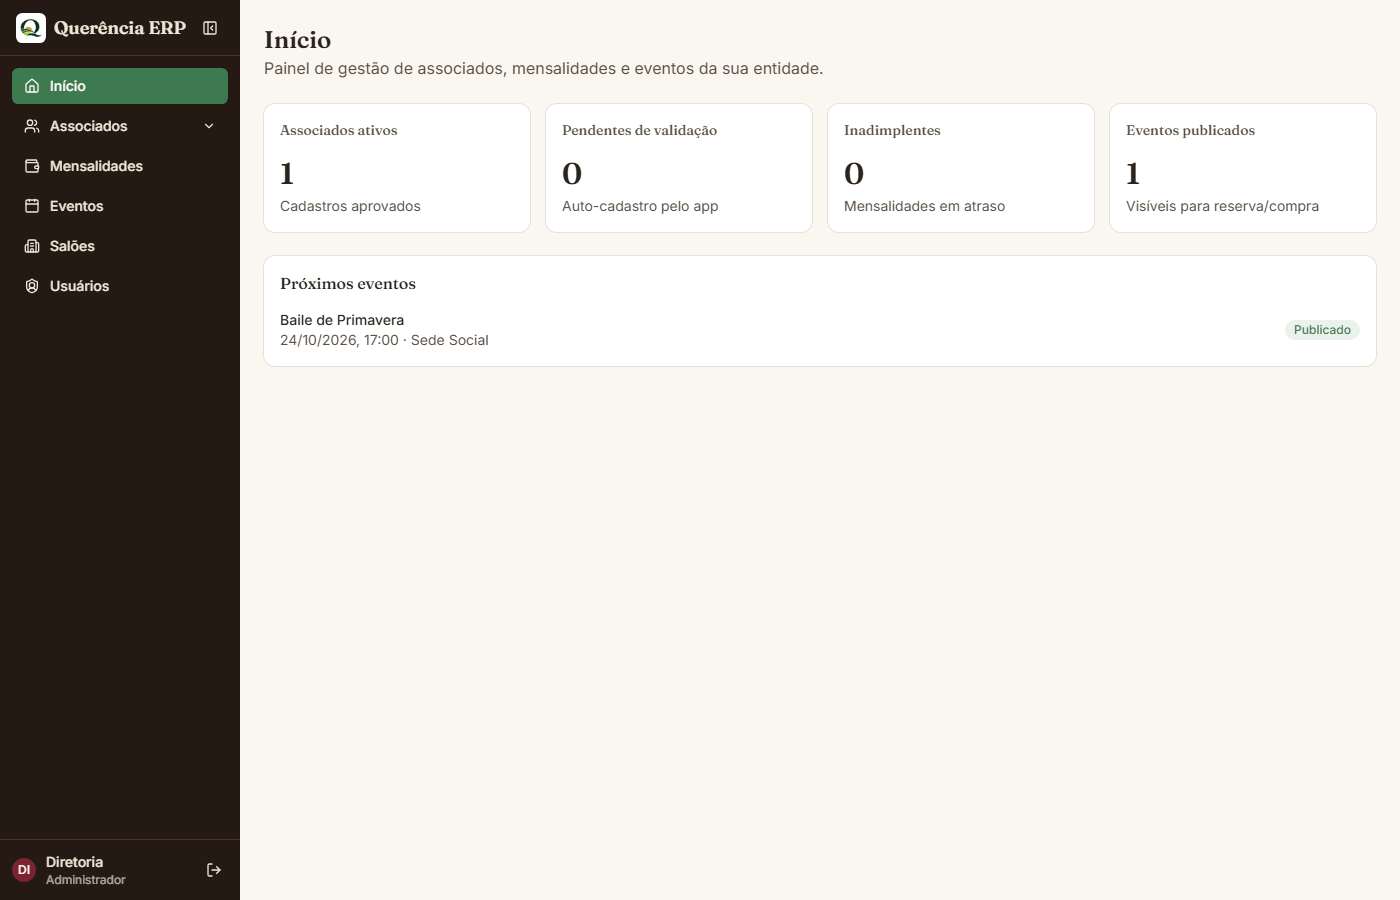
\includegraphics[width=0.92\textwidth]{figuras/web-dashboard.png}
  \caption{Painel administrativo: tela inicial}
  \label{fig:web-dashboard}
  \caption*{\textbf{Fonte:} Elaborado pelo autor (2026).}
\end{figure}

\begin{figure}[H]
  \centering
  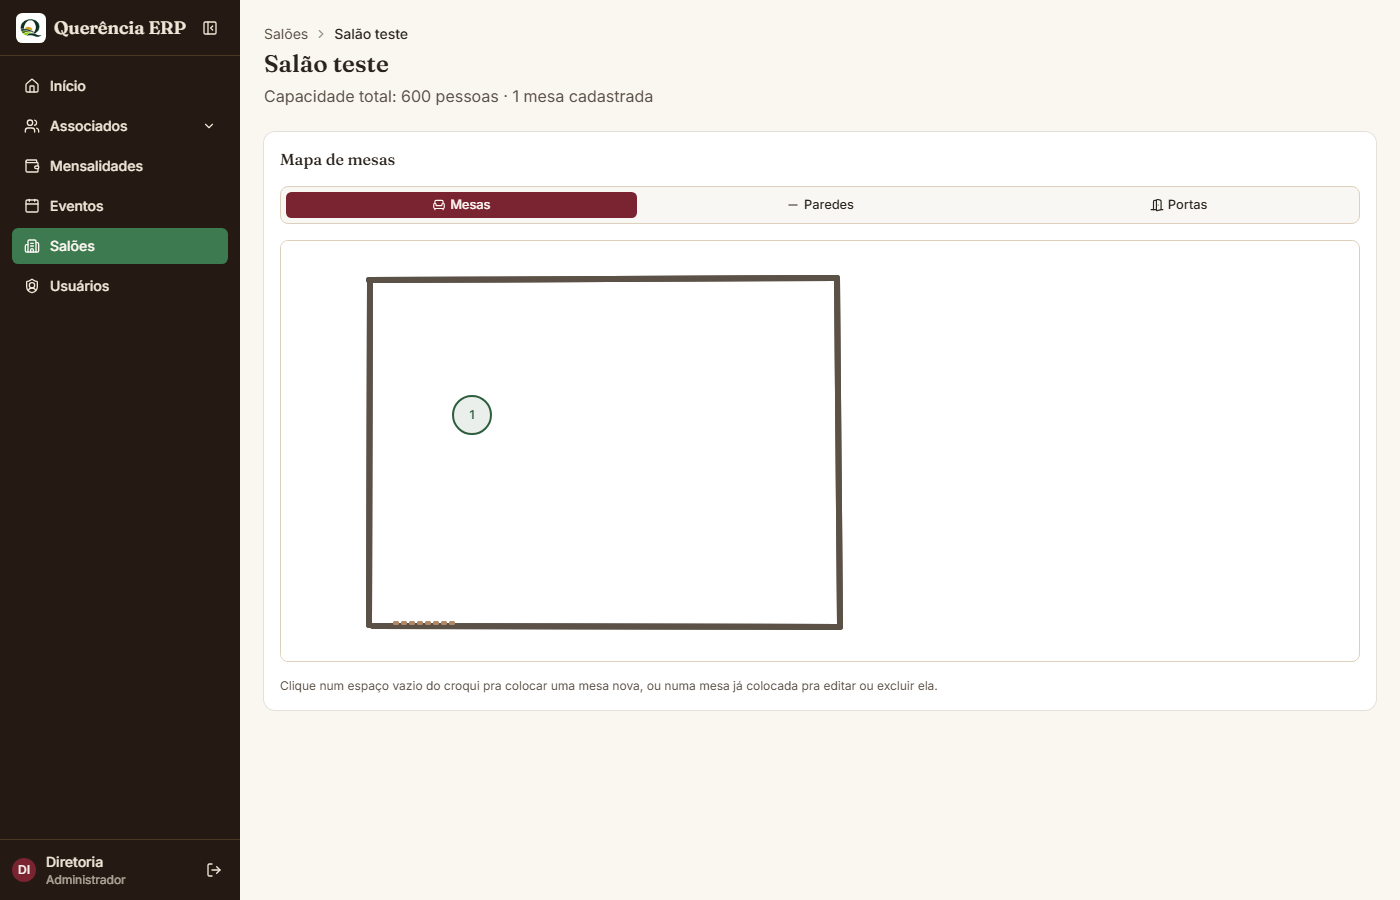
\includegraphics[width=0.92\textwidth]{figuras/web-salao-croqui.png}
  \caption{Painel administrativo: croqui do salão com mesas, paredes e portas}
  \label{fig:web-croqui}
  \caption*{\textbf{Fonte:} Elaborado pelo autor (2026).}
\end{figure}

\begin{figure}[H]
  \centering
  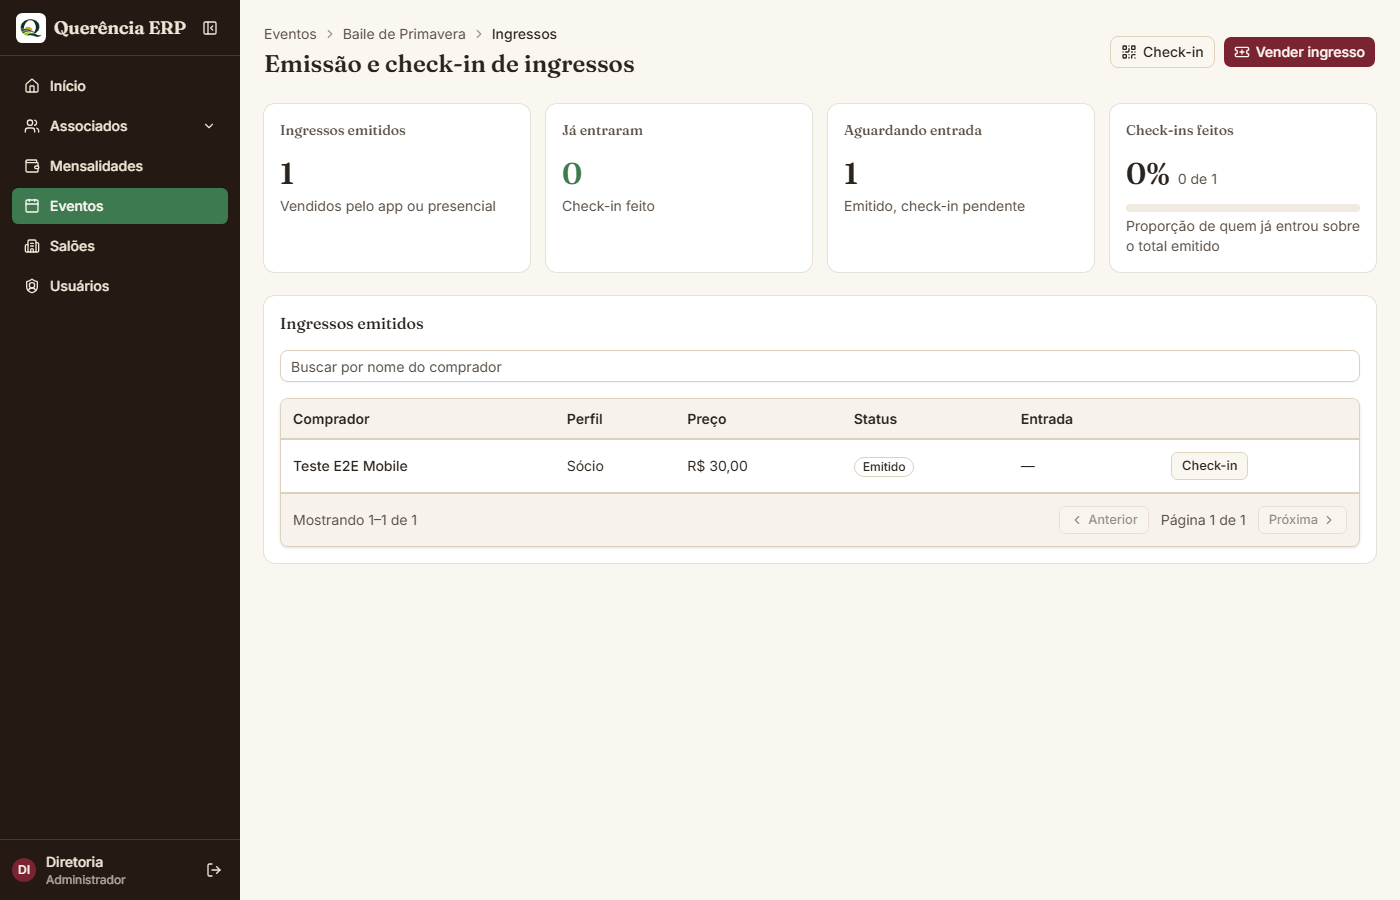
\includegraphics[width=0.92\textwidth]{figuras/web-ingressos.png}
  \caption{Painel administrativo: acompanhamento de ingressos e check-in do evento}
  \label{fig:web-ingressos}
  \caption*{\textbf{Fonte:} Elaborado pelo autor (2026).}
\end{figure}

\textbf{Aplicativo do associado (React Native + Expo).} O aplicativo oferece cinco áreas, acessadas por
uma barra de navegação inferior (Figura~\ref{fig:mobile-telas}): o início, com os dados cadastrais e a
situação do associado; as mensalidades, com o histórico e o pagamento online da cobrança em aberto; as
reservas de mesa; os ingressos; e os eventos publicados, com o mapa de mesas em tempo real e a
possibilidade de reservar uma mesa ou comprar o ingresso. O associado também pode criar a própria
conta ou vincular-se a um cadastro já feito pela diretoria. Na área de ingressos, cada ingresso
emitido é apresentado com o código QR, que a portaria lê para validar a entrada; uma vez validado,
o ingresso passa a indicar a entrada já registrada. O conteúdo do código é o identificador do
próprio ingresso, o mesmo valor aceito pelo painel na leitura por câmera ou na digitação manual, de
modo que os dois formatos de validação convivem, como previsto no levantamento de requisitos.

\begin{figure}[H]
  \centering
  \begin{minipage}[t]{0.23\textwidth}
    \centering
    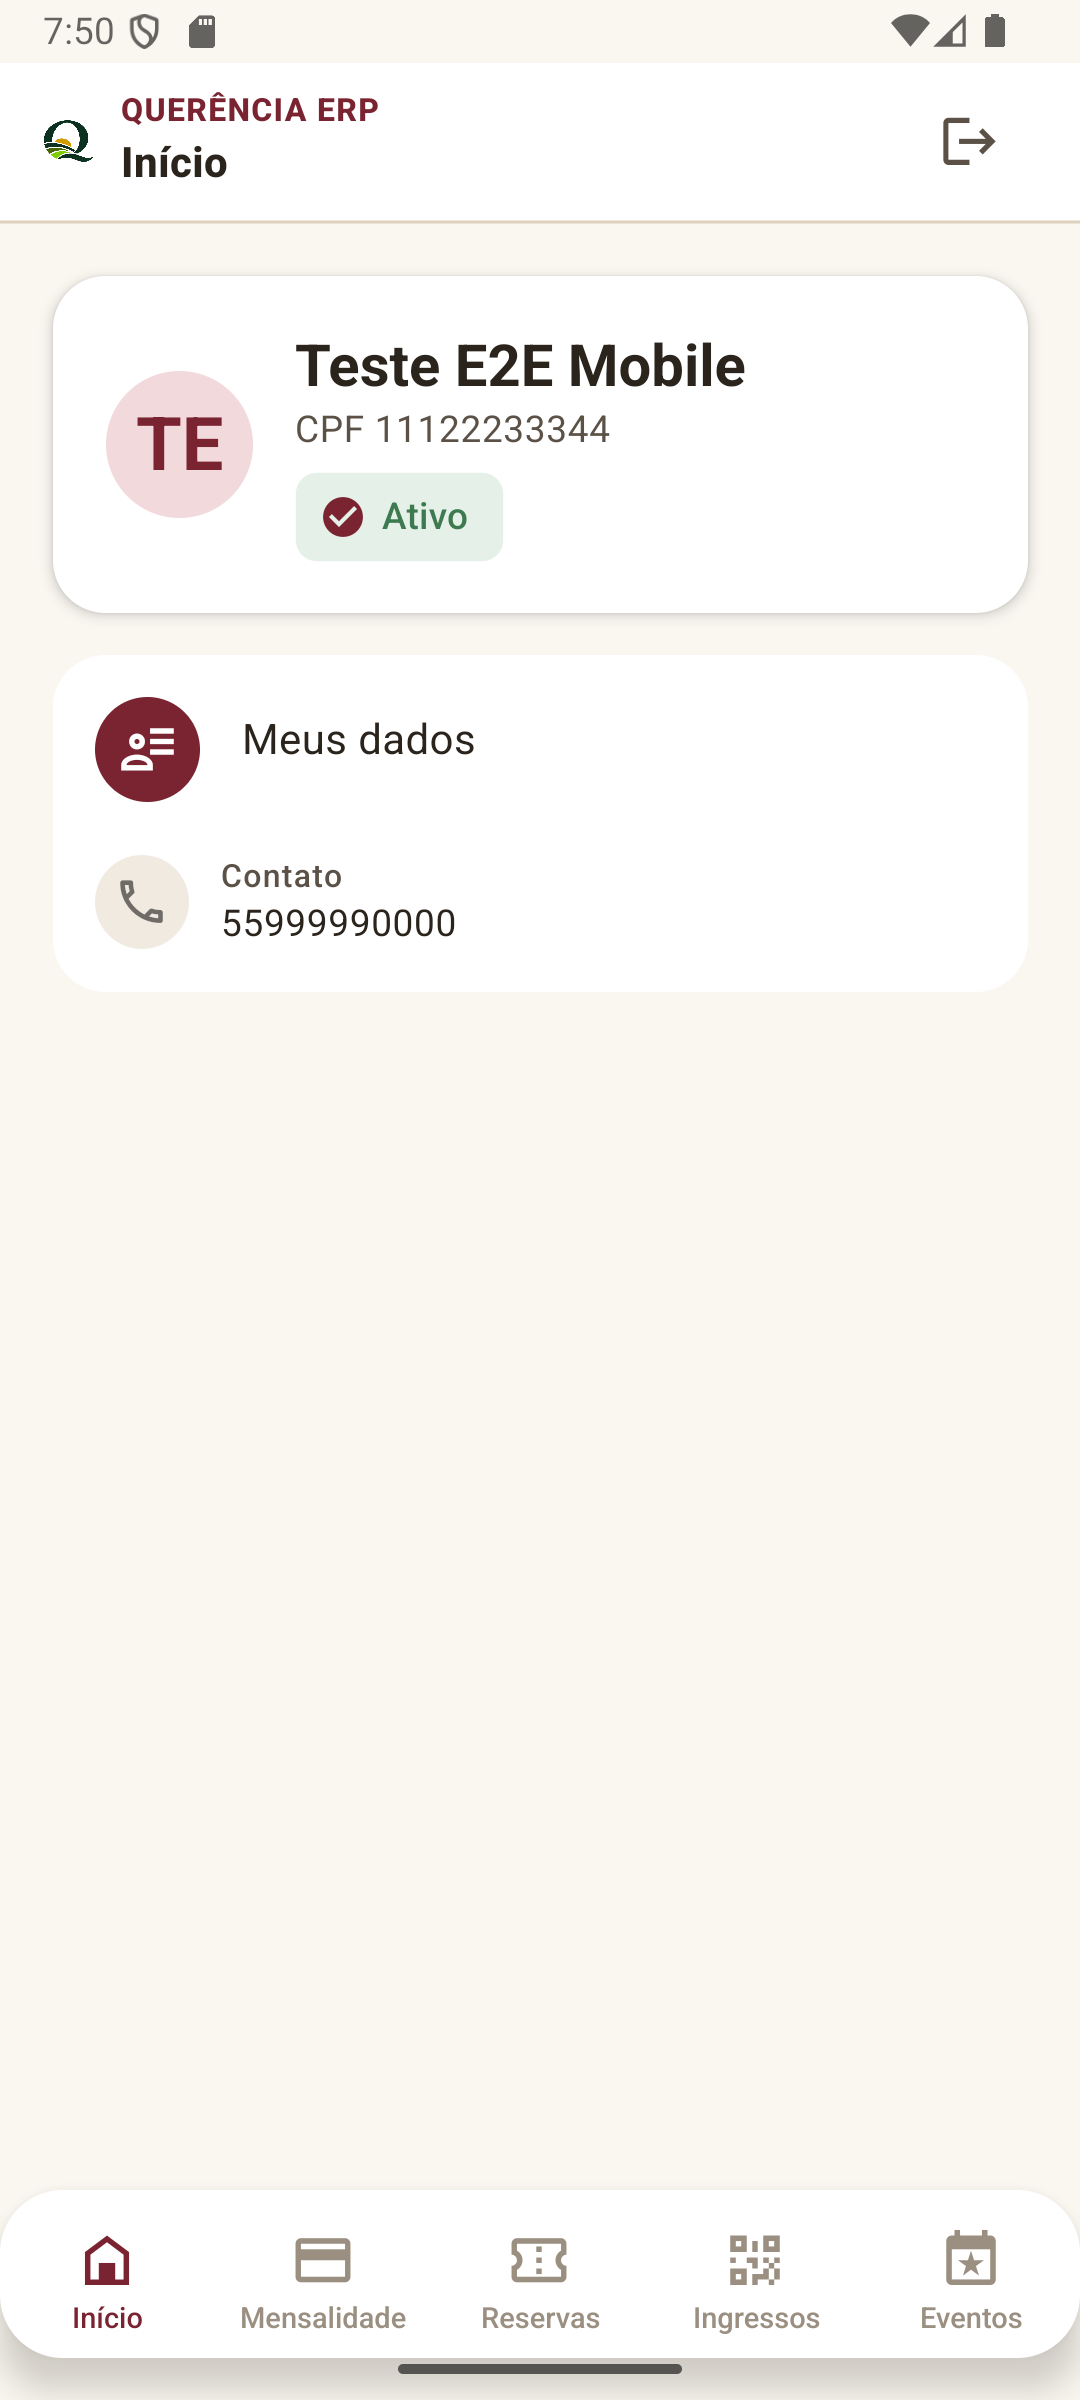
\includegraphics[width=\textwidth]{figuras/mobile-inicio.png}\\[2pt]{\small (a) Início}
  \end{minipage}\hfill
  \begin{minipage}[t]{0.23\textwidth}
    \centering
    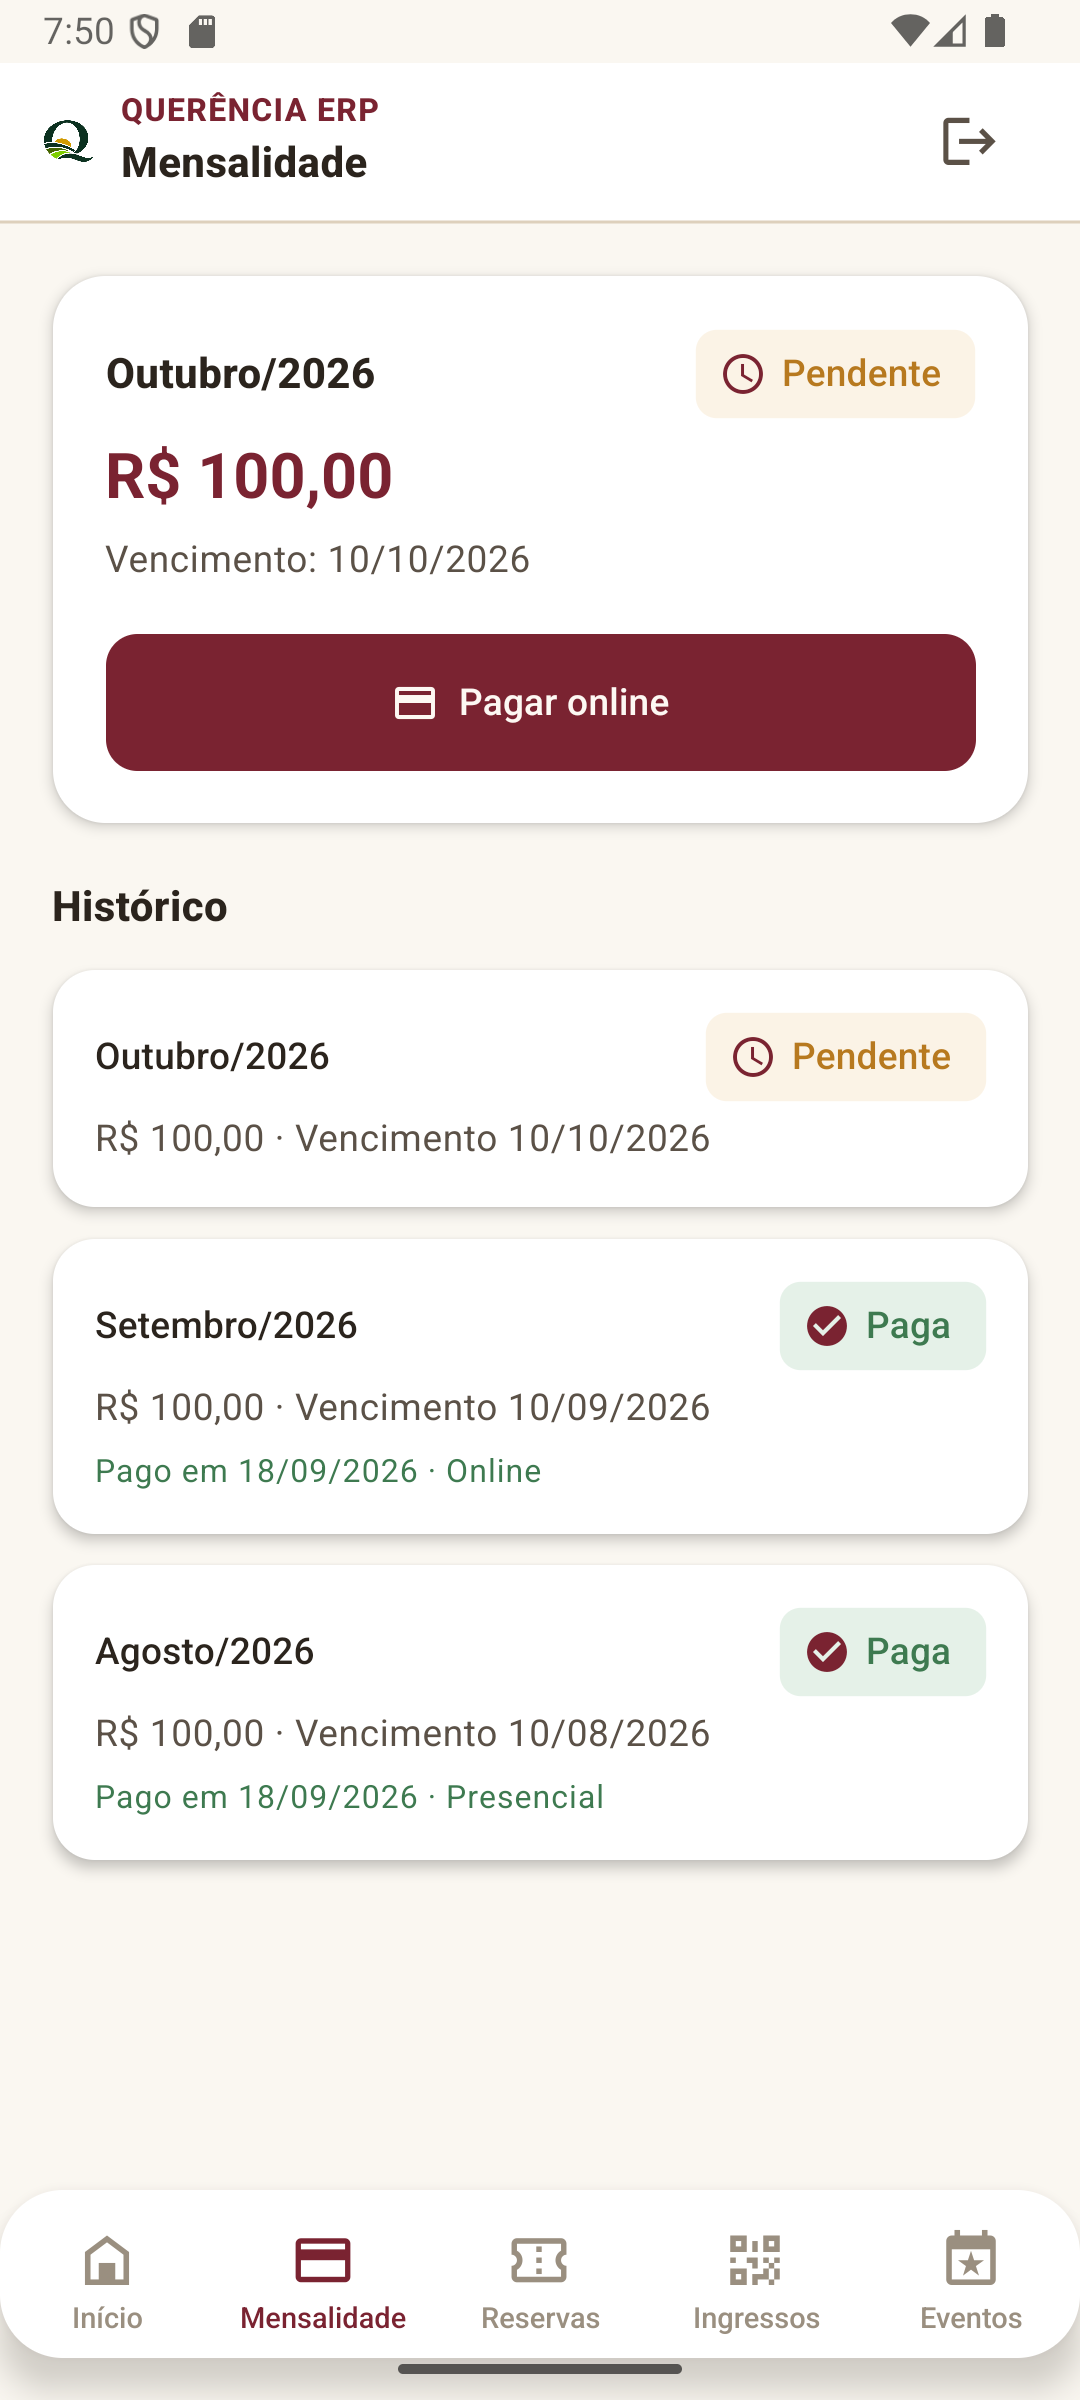
\includegraphics[width=\textwidth]{figuras/mobile-mensalidade.png}\\[2pt]{\small (b) Mensalidade}
  \end{minipage}\hfill
  \begin{minipage}[t]{0.23\textwidth}
    \centering
    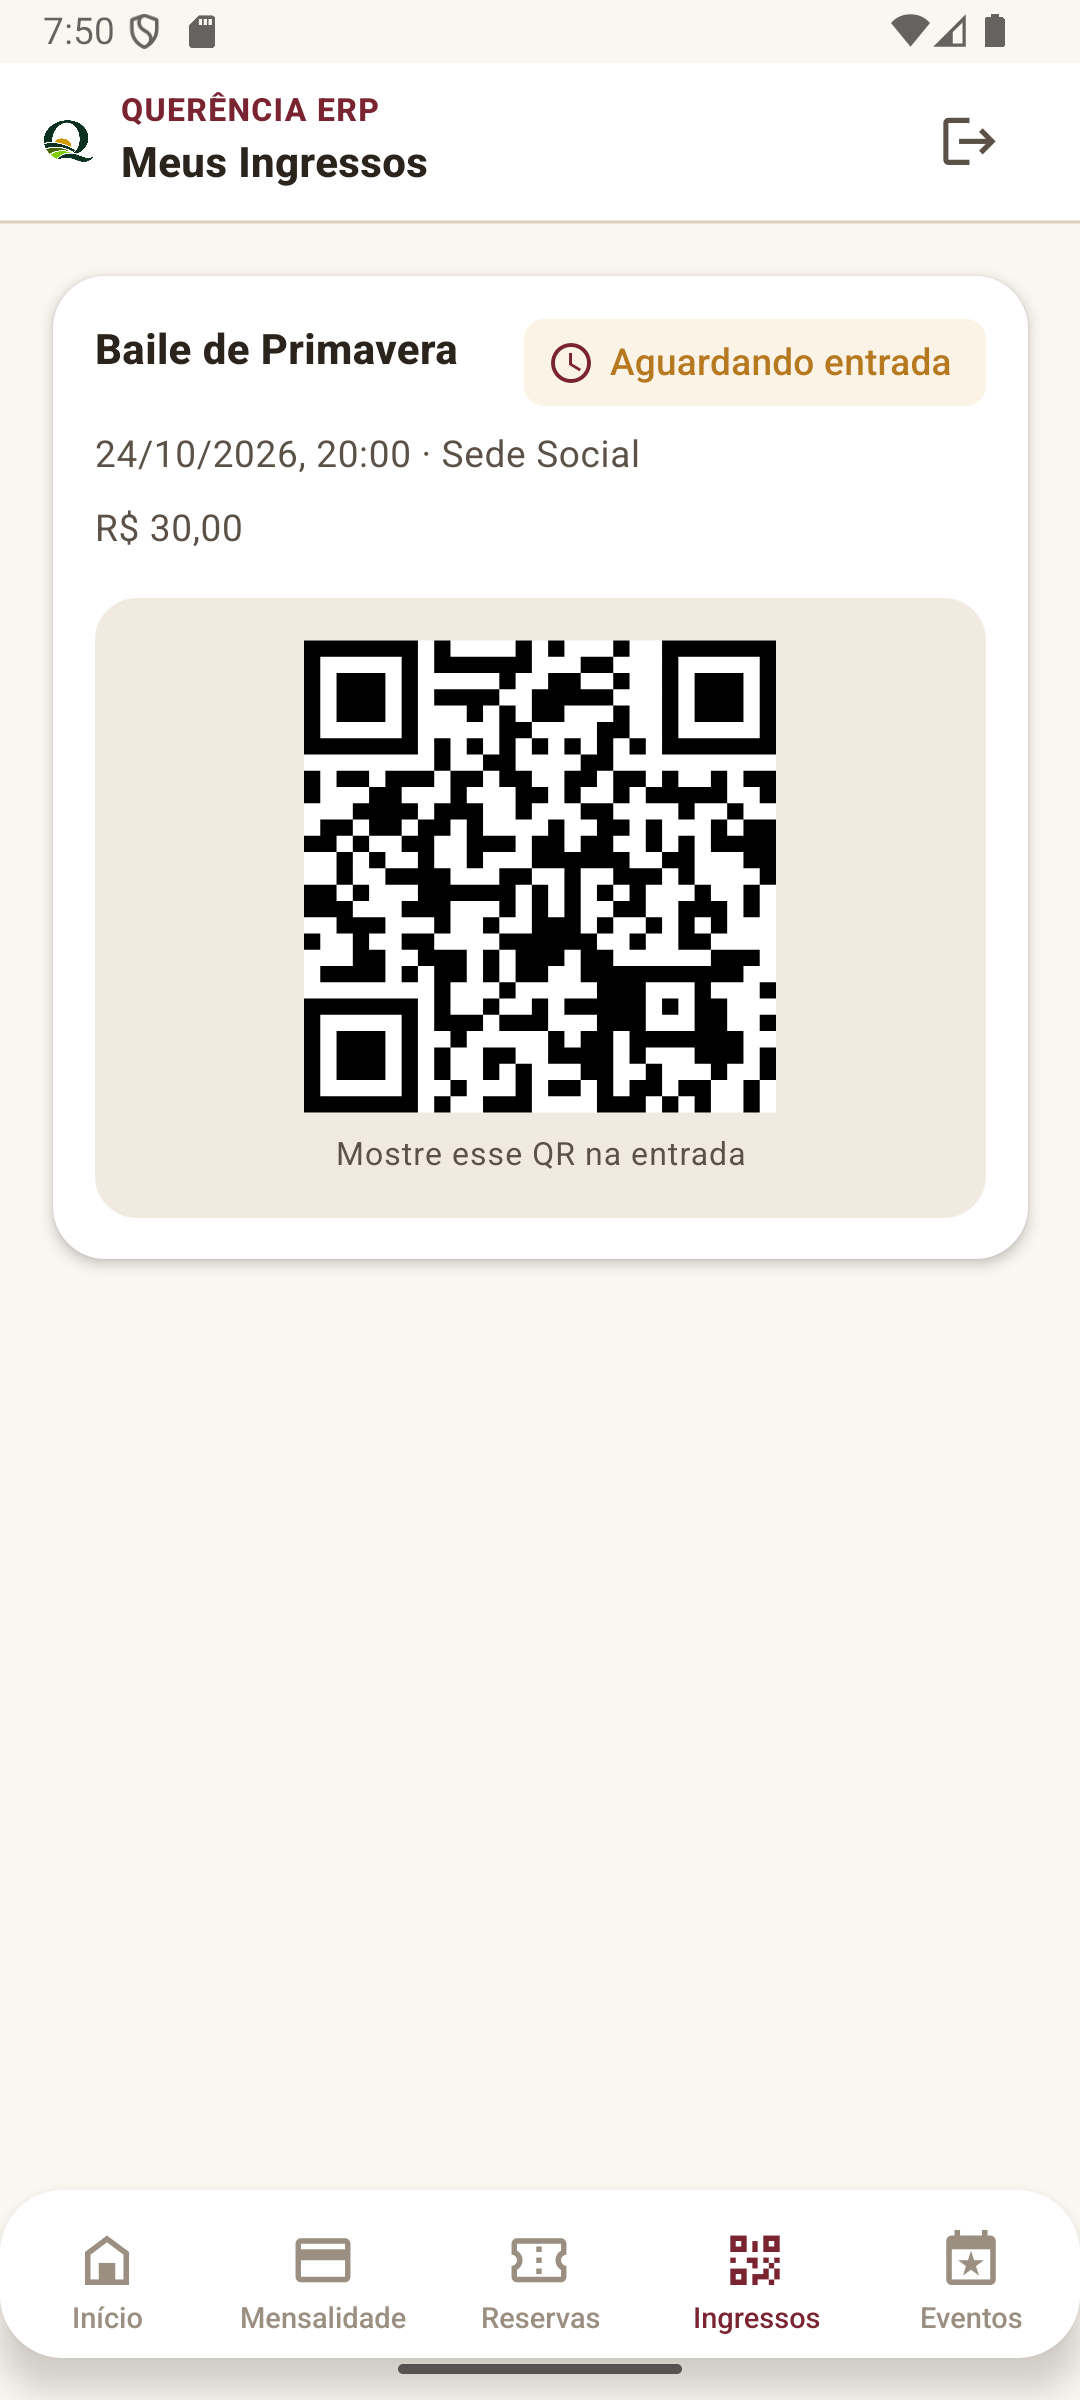
\includegraphics[width=\textwidth]{figuras/mobile-ingressos.png}\\[2pt]{\small (c) Ingressos}
  \end{minipage}\hfill
  \begin{minipage}[t]{0.23\textwidth}
    \centering
    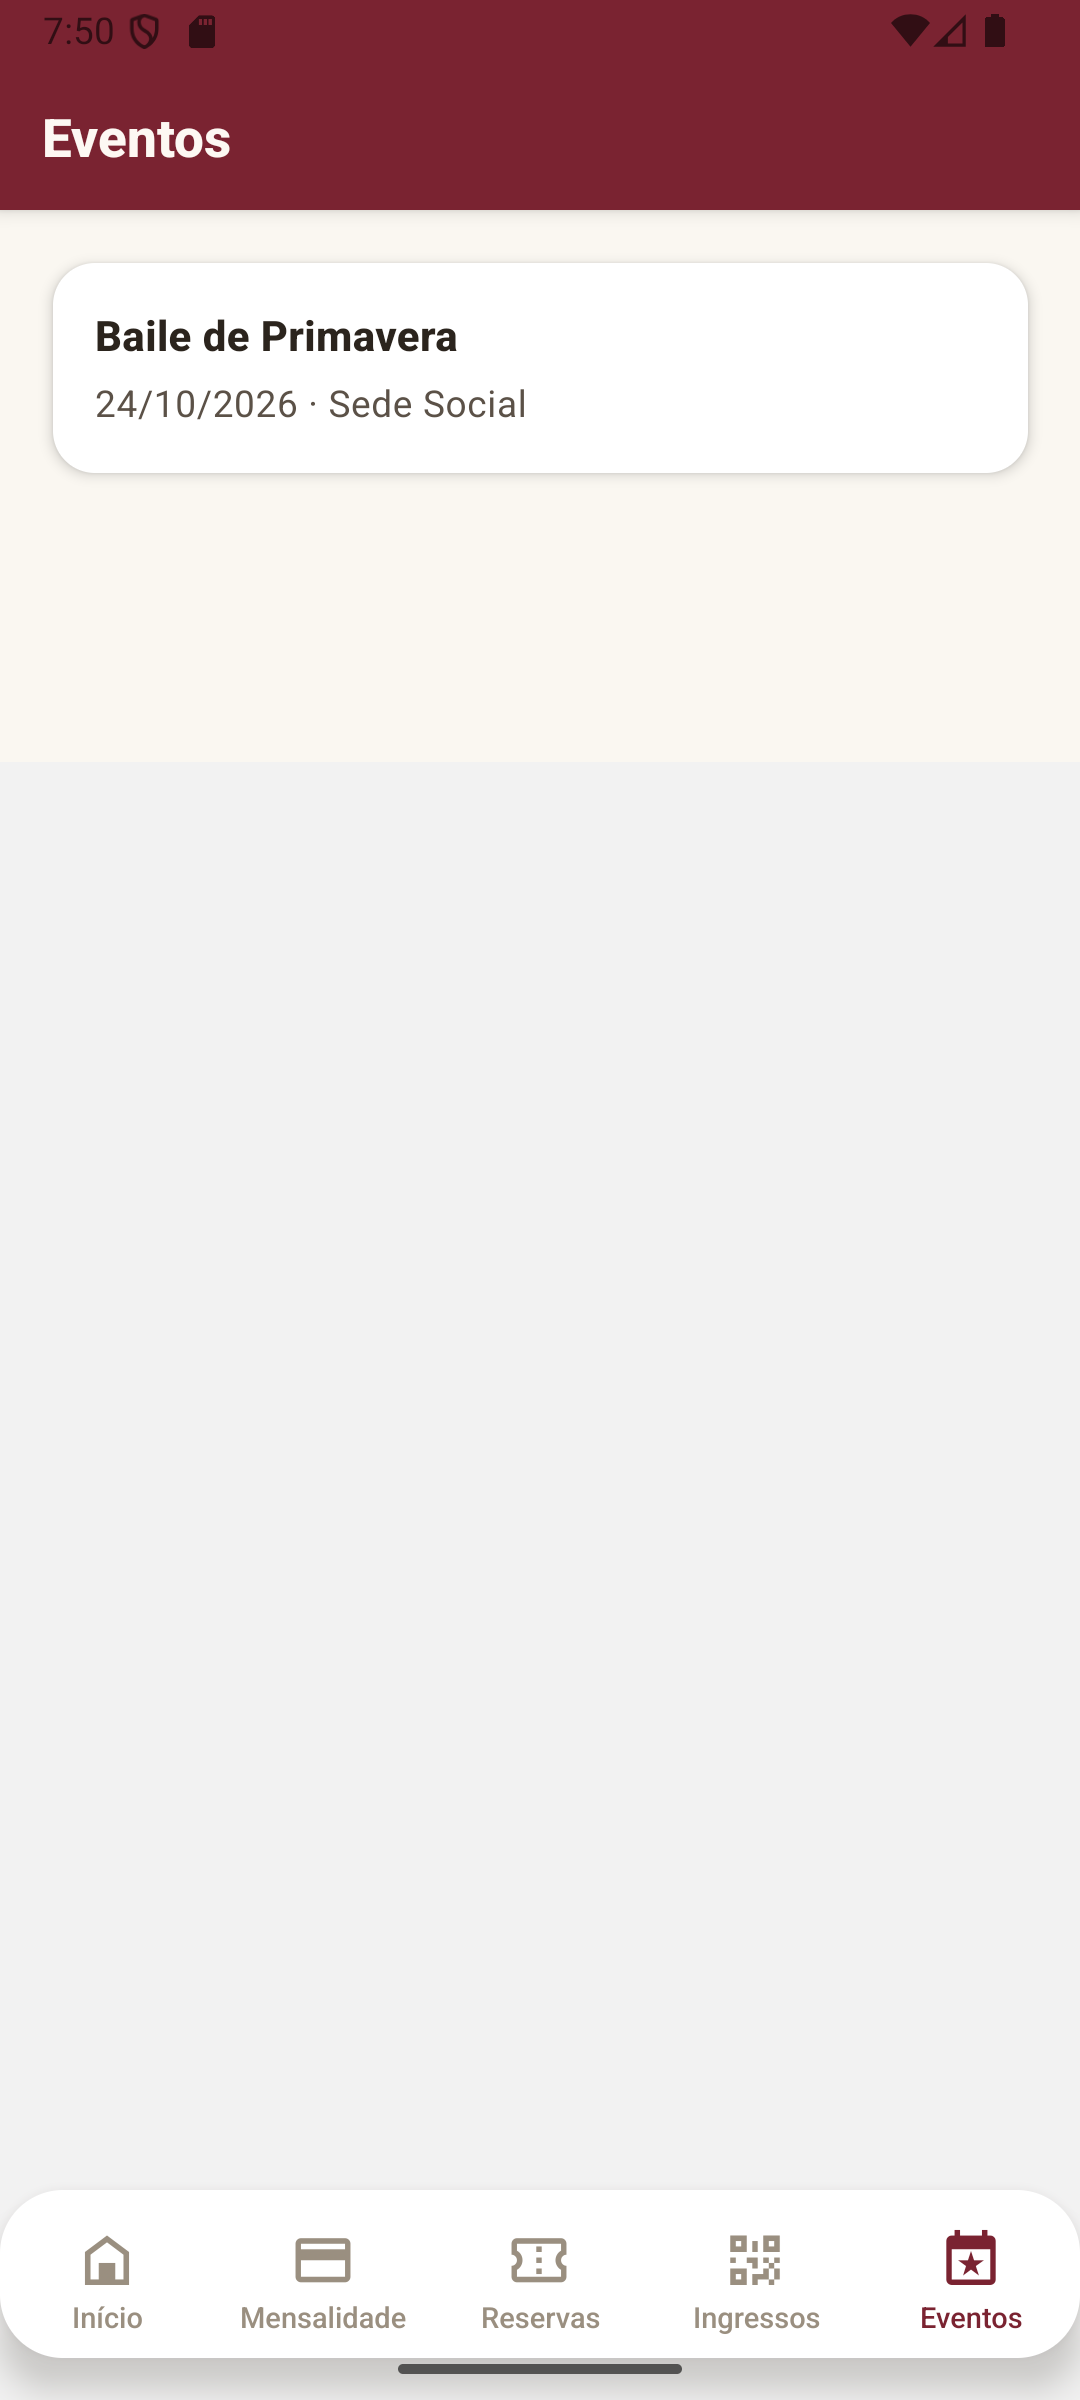
\includegraphics[width=\textwidth]{figuras/mobile-eventos.png}\\[2pt]{\small (d) Eventos}
  \end{minipage}
  \caption{Aplicativo do associado: principais telas}
  \label{fig:mobile-telas}
  \caption*{\textbf{Fonte:} Elaborado pelo autor (2026).}
\end{figure}

\textbf{Identidade visual e reutilização.} Como o sistema foi concebido para atender mais de uma
entidade, a interface não carrega o nome de nenhuma delas: o produto recebeu a identidade própria
Querência ERP (QERP), com marca criada especificamente para o projeto, aplicada de forma consistente no
painel, no aplicativo e nos ícones. As categorias de sócio, os valores de mensalidade e de ingresso
e o croqui do salão são dados configurados por cada entidade, e não regras fixas no código.

\textbf{Implantação.} A API e o painel web foram publicados como dois serviços em contêineres na
plataforma de computação em nuvem \textit{Google Cloud Run}, com o banco de dados PostgreSQL mantido em
um serviço gerenciado externo e os segredos (chave de assinatura dos tokens e cadeia de conexão com o
banco) armazenados no \textit{Secret Manager}, e não em variáveis de ambiente em texto puro. O
aplicativo foi empacotado como arquivo APK de distribuição interna por meio do serviço de compilação
\textit{Expo Application Services} (EAS), apontando para a API em produção, o que permitiu a
instalação em dispositivos Android para a validação com usuários. Cada entidade parceira poderá
operar uma instância própria a partir do mesmo código-base, sem compartilhamento de dados entre elas.

\textbf{Achados durante a implementação.} Duas lacunas foram identificadas apenas com o uso dos
protótipos, o que reforça o caráter iterativo do método. A primeira foi a ausência de vínculo entre o
ingresso e o associado que o comprou: o registro guardava somente o nome do comprador, o que
impossibilitava ao aplicativo apresentar ``os ingressos do associado''; a correção exigiu uma nova
migração do esquema e uma rota específica para o perfil de associado. A segunda foi a ausência, no
aplicativo, de qualquer forma de reabrir o ingresso após a compra, o que inviabilizava o fluxo de
validação por código QR na portaria, motivação central do sistema; a área de ingressos descrita
acima resolveu essa lacuna.

\textbf{Limitações.} Ressalvam-se os seguintes pontos: (i) a cobrança online utiliza uma
implementação simulada da porta de pagamento, sem integração com um provedor real; (ii) a reserva de
mesa é registrada para a mesa inteira, sem controle de entrada por pessoa, ao passo que a validação
na portaria por código QR está implementada apenas para o ingresso avulso, de modo que o controle de
acesso associado à reserva permanece como trabalho futuro; (iii) o aplicativo foi validado em
dispositivo Android, sem verificação em iOS; e (iv) não foi realizada aferição sistemática do tempo de
resposta (RNF05).


\subsection{Avaliação com usuários e análise dos resultados}

[Seção a ser desenvolvida após a avaliação junto às entidades parceiras. Apresentará os resultados do
SUS, as percepções coletadas nas entrevistas, os registros de observação e a análise qualitativa com
triangulação dos dados, discutindo pontos de convergência e de divergência entre o CPF Pia do Sul e o
CTG Sentinela da Querência. Discutirá as contribuições e limitações do sistema em relação ao contexto
identificado.]

% ------------------------------------------------------------------
\section{Considerações finais}
% ------------------------------------------------------------------

[Seção a ser desenvolvida ao final do trabalho. Retomará o problema de pesquisa e os objetivos,
apresentará as conclusões sustentadas pelos resultados, explicitará as contribuições sociais, práticas
e científicas, as limitações da pesquisa e recomendações para trabalhos futuros.]

Esta pesquisa buscou responder à seguinte questão: como um ecossistema digital integrado pode
facilitar e qualificar a gestão de associados e eventos sociais em entidades tradicionalistas
gaúchas, respeitando suas especificidades culturais e organizacionais? A resposta a essa pergunta
será construída a partir da avaliação empírica conduzida junto às duas entidades parceiras, o CPF Pia
do Sul e o CTG Sentinela da Querência, articulada com a fundamentação teórica sobre sistemas de
informação, ecossistemas digitais e transformação digital em organizações culturais.

Como contribuição acadêmica, espera-se demonstrar a viabilidade de aplicação de um ecossistema
digital em contextos culturais tradicionais, evidenciando que modernização administrativa e
preservação das dinâmicas culturais podem coexistir de forma complementar
\parencite{hinings2018,vial2019}.

% Inclua na bibliografia apenas as obras efetivamente citadas no texto.
\printbibliography[title={REFERÊNCIAS}]

\end{document}
